\documentclass[
  digital, %% This option enables the default options for the
           %% digital version of a document. Replace with `printed`
           %% to enable the default options for the printed version
           %% of a document.
  notable, %% Causes the coloring of tables. Replace with `notable`
           %% to restore plain tables.
  lof,     %% Prints the List of Figures. Replace with `nolof` to
           %% hide the List of Figures.
  lot,     %% Prints the List of Tables. Replace with `nolot` to
           %% hide the List of Tables.
  nopalatino, color
  %% More options are listed in the user guide at
  %% <http://mirrors.ctan.org/macros/latex/contrib/fithesis/guide/mu/fi.pdf>.
]{fithesis3}
\usepackage[resetfonts]{cmap} %% We need to load the T2A font encoding
\usepackage[T1,T2A]{fontenc}  %% to use the Cyrillic fonts with Russian texts.
\usepackage[
  main=english, %% By using `czech` or `slovak` as the main locale
                %% instead of `english`, you can typeset the thesis
                %% in either Czech or Slovak, respectively.
  czech         %% The additional keys allow
]{babel}        %% foreign texts to be typeset as follows:
%%
%%   \begin{otherlanguage}{german}  ... \end{otherlanguage}
%%   \begin{otherlanguage}{russian} ... \end{otherlanguage}
%%   \begin{otherlanguage}{czech}   ... \end{otherlanguage}
%%   \begin{otherlanguage}{slovak}  ... \end{otherlanguage}
%%
%% The following section sets up the metadata of the thesis.
\thesissetup{
    date          = 2017/12/13,
    university    = mu,
    faculty       = fi,
    type          = mgr,
    author        = Vít Novotný,
    gender        = m,
    assignment    = {misc/assignment},
    advisor       = {Doc. RNDr. Petr Sojka, Ph.D.},
    title         = Vector Space Representations in Information Retrieval,
    keywords      = {document segmentation, synonymy, question answering, vector space model, 
                     text retrieval, information retrieval},
    abstract      = {Modern text retrieval systems employ text segmentation
                     during the indexing of documents. I show that, rather than
                     returning the segments to the user, significant
                     improvements are achieved on the semantic text similarity
                     task by combining all segments from a single document into
                     one result with an aggregate similarity score. 

                     Standard text retrieval methods underestimate the semantic
                     similarity between documents that use synonymous terms.
                     Latent semantic indexing tackles the problem by clustering
                     frequently co-occuring terms at the cost of the periodical
                     reindexing of dynamic document collections and the
                     suboptimality of co-occurences as a measure of synonymy.
                     I develop a term similarity model that suffers neither of
                     these flaws.},
    thanks        = {I wish to express my most sincere gratitude to my thesis
                     supervisor, Petr Sojka, for sharing his impeccable
                     expertise, valuable guidance, and for introducing me to
                     the larger scientific community.\bigskip

                     \noindent I would also like to thank Radim Řehůřek who
                     provided me with countless thought-provoking insights
                     during my work on the thesis.\bigskip

                     \noindent I would also like to thank my parents for their
                     unceasing encouragement and support during my
                     studies.\bigskip

                     \noindent Lastly, I wish to express my sincere thanks to
                     all those who have helped me, either directly or
                     indirectly, in cultivating the ideas presented in this
                     thesis.},
    bib           = {main.bib, sojka.bib},
}
\usepackage{makeidx}      %% The `makeidx` package contains
\makeindex                %% helper commands for index typesetting.
%% These additional packages are used within the document:
\usepackage[proportional,osf]{newpxtext}
\usepackage{mathpazo}
\usepackage[T1]{fontenc}
\usepackage{amsmath,amssymb}
\usepackage{array}
\usepackage{tikz}
\usetikzlibrary{positioning,fit,shapes,arrows}
\usepackage{booktabs}
\usepackage{xparse}
\usepackage{xspace}
\usepackage{rotating}
\usepackage{placeins}
\usepackage{floatpag}
\rotfloatpagestyle{plain}
\PassOptionsToPackage{maxcitenames=2}{biblatex}
%% These additional commands are used within the document:
\newenvironment{liningfigs}{\renewcommand*{\rmdefault}{zpltlf}\normalfont}{}
\newif\ifthesis\thesistrue
\newif\ifdebug\debugtrue
\newif\iflong\longtrue
\newif\ifreview\reviewfalse
\newcommand*\rot{\rotatebox{70}}
\newcommand{\op}[1]{\ensuremath{\operatorname{#1}}}
\newcommand{\avg}{\op{avg}}
\newcommand{\wavg}{\op{wavg}}
\newcommand{\sign}{\op{sign}}
\newcommand{\etal}{\unskip~\textit{et\penalty100\ al.}\xspace}
\newcommand{\longsubsection}[1]{\iflong\subsection{#1}\fi}
\def\abbr#1{\textsc{\MakeLowercase{#1}}}
\let\term\emph
\newcommand{\omid}{\rotatebox[origin=c]{-90}{$\ominus$}}
\makeatletter
\newcommand*{\bigominus}{\DOTSB\bigominus@\slimits@}
\newcommand{\bigominus@}{\mathop{\mathpalette\bigominus@@\relax}}
\newcommand{\bigominus@@}[2]{%
  \vcenter{\hbox{%
    \sbox\z@{$\m@th#1\bigoplus$}%
    \resizebox{\wd\z@}{!}{$\m@th#1\ominus$}%
  }}%
}
\makeatother
\newcommand{\bigomid}{\rotatebox[origin=c]{-90}{$\bigominus$}}
\NewDocumentCommand\todo{ggo}{%
  \ifdebug
    \textcolor{red}{TODO}%
    \IfValueT{#1}{\textcolor{red}{:~}}%
    \IfValueT{#1}{\textcolor{blue}{#1}}\nopagebreak%
    \IfValueT{#2}{\\\textcolor{orange}{#2}}\nopagebreak%
    \IfValueT{#3}{\\\textcolor{magenta}{#3}}%
  \fi}
% \done has the same args as \todo
\NewDocumentCommand\done{ggo}{%
  \ifdebug
    \textcolor{green}{DONE}%
    \IfValueT{#1}{\textcolor{green}{:~}}%
    \IfValueT{#1}{\textcolor{blue}{\sout{#1}}}\nopagebreak%
    \IfValueT{#2}{\\\textcolor{orange}{\sout{#2}}}\nopagebreak%
    \IfValueT{#3}{\\\textcolor{magenta}{\sout{#3}}}%
  \fi}
\newcommand*{\tran}{^{\mkern-1.5mu\mathsf{T}}}
\let\note=\footnote
\hyphenation{Wiki-pe-dia}
%% These additional packages that are used in the document need to be loaded
\thesisload %% after the fithesis style files:
\usepackage{bm}
%% These additional commands that are used in the document need to be defined
\thesisload %% after the fithesis style files have been loaded:
\let\emph=\textit
\let\subsubsection=\paragraph
\makeatletter\let\ps@headings=\relax\makeatother
\begin{document}

\chapter{Introduction}
In 2012, a study conducted by the International Data
Corporation (\abbr{IDC}) predicted that by the year 2020, the total amount of
digital information resources will have reached the 40 zettabyte
mark~\cite{gantz2012digital}. According to the rule formulated
by~\citefield{shilakes1998enterprise}{journaltitle}, $80$ to $90$\,\% of these
resources will be unstructured.~\cite{shilakes1998enterprise} Despite the large
amount of unstructured information, users expect an information retrieval
(\abbr{IR}\index{ir@\abbr {IR}|emph}) system to be both fast and accurate with
respect to their information need. Due to these demands,
\abbr{IR}\index{ir@\abbr {IR}} remains an active field of information science
more than half a century after Calvin Mooers first formulated its
principles~\cite{mooers1950information}.

As a researcher in the Math Information Retrieval (\abbr{MIR})
group\note{\url{https://mir.fi.muni.cz/}} at the Masaryk University in Brno,
Czech Republic, I participated in a state-funded research project in
collaboration with a research team from RaRe
Technologies\note{\url{https://rare-technologies.com/}}. The goal of the
project was to develop a text retrieval system that would incorporate the
state-of-the-art research in \abbr{IR}\index{ir@\abbr {IR}} while remaining
efficient. During the project, I was given an opportunity to attend the 55th
Annual Meeting of the Association for Computational Linguistics
(\abbr{ACL}\index{acl@\abbr{ACL}|emph}) in Vancouver, Canada, where I presented
our research~\cite{rygletal17} along with my thesis supervisor. In reaction to
our research and other work presented at \abbr{ACL}\index{acl@\abbr{ACL}}~2017,
I formulated and carried out two experiments that are the subject of this work.

In my experiments, I used the question answering
(\abbr{QA})~\index{qa@\abbr{QA}|emph} datasets developed for the third task of
the 10th and 11th International Workshop on Semantic Evaluation (SemEval).
I describe the properties of these datasets in chapter~\ref{chap:datasets}.

The system we developed splits the stored documents into semantically coherent
segments~\cite{rygletal16}. One of the major advantages of this approach is
that short and highly relevant sections are retrieved rather than whole
documents that often cover a multitude of topics irrelevant to the user. In
practice, text \abbr{IR}\index{ir@\abbr {IR}} systems rarely have this amount of
leeway and are required to present the whole documents in the search results.
In my first experiment described in chapter~\ref{chap:segmentation}, I show
that even such systems can improve their performance on the text similarity
task by using segmentation internally.

Today's text \abbr{IR}\index{ir@\abbr {IR}} systems are largely based on the
standard vector space bag-of-words model first described by
\textcite{ir:Salton1975}\index{standard model}\index{bag of words|see{standard
model}}. This model is simple and well-understood, but it makes the assumption
that concepts described by different terms are unrelated. In reaction to the
work of \textcite{charletdamnati17} that was published and presented at
\abbr{ACL}\index{acl@\abbr{ACL}}~2017, I developed an extension to the standard
model that exploits term synonymy. In my second experiment described in
chapter~\ref{chap:synonymy}, I explore several properties of the extended
model\index{standard model!extended} and show that the extension improves the
performance of the standard model on the text similarity task.

Both chapters~\ref{chap:segmentation} and \ref{chap:synonymy} are structured as
self-contained full papers with their own introduction and conclusion sections.
The experimental code in Python for both experiments is publicly
available\note{\url{https://github.com/witiko-masters-thesis}}. In the code, I
make abundant use of the \abbr{GNU}~Parallel~\cite{Tange2011a},
Gensim~\cite{rehurek_lrec}, and SciPy~\cite{scipy} software packages.

I conclude this work in chapter~\ref{chap:conclusion} by summarizing the
results of both experiments, giving a perspective on how the ideas developed in
chapters~\ref{chap:segmentation} and \ref{chap:synonymy} can be used together
in a single system, and suggesting future work.

\chapter{Datasets}
\label{chap:datasets}
In my experiments, I evaluated the systems on the SemEval-2016 and 2017
task~3 subtask~B question answering (\abbr{QA})\index{qa@\abbr{QA}} datasets.
These datasets consist of discussion threads from the Qatar
Living\note{\url{http://www.qatarliving.com/forum}} internet forum. Given
an original question, and a set of ten candidate threads containing both a
related question and the initial ten comments in the thread, the task is to
rank the candidate threads by their relevance to the original
question.~\cite{preslavetal16,nakov2017semeval} The performance of a system
is evaluated by its mean average precision\index{map@\abbr {MAP}|emph}
(\abbr{MAP}) using relevance judgements.

The SemEval-2016 task~3 subtask~B datasets consist of the training dataset (267
original questions, 1,790~threads), the dev dataset (50~original questions,
244~unique threads), and the test dataset (70~original questions, 327~unique
threads). The winning SemEval-2016 task~3 subtask~B submission was
\term{\abbr{UH-PRHLT}-primary} with a \abbr{MAP}\index{map@\abbr {MAP}} score of
$76.7$. SemEval-2017 task~3 subtask~B uses the same training and dev datasets as
SemEval-2016 with the provision that the SemEval-2016 test dataset can be used
for training. A new test dataset (88 original questions, 293 unique threads)
has also been added.  The SemEval-2017 task~3 subtask~B winning configuration
was \term{SimBow-primary} with a \abbr{MAP}\index{map@\abbr {MAP}} score of $47.22$.

I also used the SemEval-2016 and 2017 task~3 subtask~A datasets for
statistical analysis. These datasets contain the same data (2,654 questions,
26,540 comments) as the subtask~B training datasets, but now the relevance
judgements assess how relevant a comment is to a question.  For language
modelling, the unannotated SemEval-2016 and 2017 task~3 subtask~A
datasets (189,941 questions, 1,894,456 comments) are available.

\section{Relevance analysis}
\label{sec:dataset-relevance-analysis}
In 1991, the American attorney and author Mike Godwin formulated%
\note{\url{news:1991Aug18.215029.19421@eff.org}} a rule that ``as a Usenet
discussion grows longer, the probability of a comparison involving Nazis or
Hitler approaches one.'' An immediate corollary would be that as an online
discussion grows longer, the probability of a relevant contribution approaches
zero. I was curious whether the datasets would confirm these observations.

I used the subtask~A relevance judgements to estimate the probability mass
function $\hat P(\textrm{at position }i\mid\textrm{relevant})$ for
$i=1,2,\ldots,10$. Since there is a uniform number of comments at each
position $i$, e.g. $\hat P(\textrm{at position }i) = 0.1$, we would expect
$\hat P(\textrm{at position }i\mid\textrm{relevant})$ to be also uniform if
the position of a comment and its relevance are independent.
Figure~\ref{fig:dataset-relevance-analysis} shows that this expectation is
false, and that there seems to be an inverse relationship between the position
of a comment and its relevance.

\begin{figure}[tb]
\centering
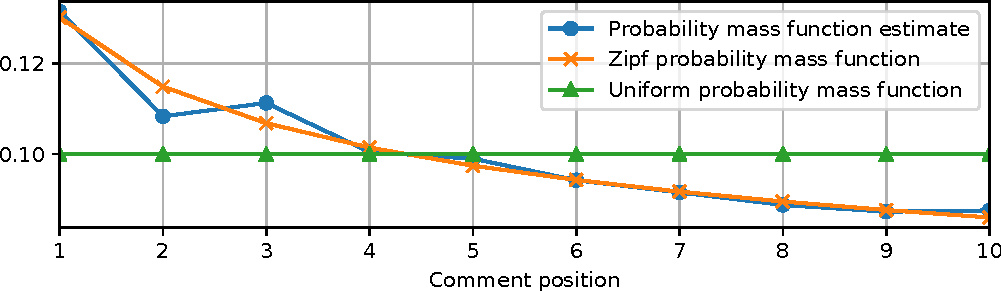
\includegraphics[trim={0cm 0cm 0cm 0cm}, scale=0.75]{figs/quality-evaluation-1}
\caption[Probability mass function estimate $\hat P(\text{at position
}i\mid\text{relevant})$]{%
  Probability mass function (\abbr{pmf}) estimate $\hat
  P(\text{at position }i\mid\text{relevant})$ plotted along the \abbr{pmf} of
  the Zipf distribution with parameters $n=10,$ and $s=0.18$.  If the position
  of a comment and its relevance were independent, we would expect the
  \abbr{pmf} estimate to be uniformly distributed.}
\label{fig:dataset-relevance-analysis}
\end{figure}

To see if this relationship was statistically significant, I modeled the number
of relevant comments at each position~$i$ as a binomial random variable
$X_i\sim \mathrm{Bi}(n, \theta_i)$ with a known number of trials $n=2{,}410$,
and an unknown probability of success $\theta_i$. I then used the one-tailed
Fisher's exact test to reject the following system of null hypotheses at 5\%
significance:
\begin{equation*}
  H_0^{(ij)} : \theta_i = \theta_j,\text{ where }i, j = 1,2,\ldots,10, i < j
\end{equation*}
I rejected $H_0^{(ij)}$ for any $j-i > 3$. Namely, I failed to reject $H_0^{(ij)}$
for $(i,j) = (2,3),$ $(4,5),$ $(5,6),$ $(6,7),$ $(7,8),$ $(7,9),$ $(7,10),$
$(8, 9),$ $(8,10)$, and $(9,10)$. The Benjamini-Hochberg procedure was used to
control the false discovery rate due to multiple testing.

\chapter{Segmented Retrieval}
\label{chap:segmentation}
% elevator pitch
% struktura dle http://www.herout.net/blog/2013/12/jak-psat-abstrakt/:
%1) Jaký se řeší problém? Jaké je téma? Jaký je cíl textu?
%řeší se problém segmentace pro přesnější indexaci a vyhledávání 
%v textech.
Modern text retrieval systems employ text segmentation during the indexing of documents.
%2) Jak je problém vyřešen? Cíl naplněn?
%problém je řešen zpřesňováním sémantické reprezentace nugetů
%a vážením nugetů dle typu databáze (Godwin)
I show that, rather than returning the segments to the user,
significant improvements are achieved on the semantic text
similarity task by combining all segments % (nuggets)
from a single document into one result with an aggregate similarity score. 
%
%3) Jaké jsou konkrétní výsledky? Jak dobře je problém vyřešen?
%
%lépe než u SemEval 2016 a 2017
Following an analysis of the SemEval-2016 and 2017 task~3 datasets, I design a
segment decay weighting method that achieves state the art results on subtask~B
and can be readily implemented into existing inverted-index-based search
engines.
%4) Takže co? Čím je to užitečné Vědě a čtenáři?
% (Nebylo zde řečeno nic nového oproti bodu 2, takže jsem text zkrátil, čímž
% dostáváme k dobru řádek.)
% Ale ztracime tim udernou shrnujici vetu, ktera bude ve vsech indexacnich databazich
% typu WoS atp. Co tedy
% Segmentation in information retrieval matters, and leads to the best results in
% QA domain.
%
% Our results show that paying attention to important segments and using a
% task-specific weighting method leads to the best results on these question
% answering domain retrieval tasks.
%
%Take off: sémantická reprezentace dobře segmentovaných, tj. význam nesoucích částí je klíčem k úspěchu. důležité je i jejich vážení a agregace/výber dle specifik dokumentové sady a aplikace. 

\section{Introduction} 
%The vector space model (VSM)~\cite{ir:Salton1975} of representing documents,
%Representations of document semantics based solely on 
%document-term statistics, such as TF-IDF or 
%\href{https://en.wikipedia.org/wiki/Okapi_BM25}{Okapi BM25}, are 
%limited in their expressiveness and search precision.
%
%%Topics (topic modeling) of representing topic of documents
%
%Distributional semantics and deep learning allow building
%of semantic vector space models (SVSM) representing words, sentences,
%paragraphs or even whole documents as vectors in high-dimensional
%spaces~\cite{nlp:LSA1990,blei03lda,ml:mikolov2013distributed}.
%
%Segmentation matters: representation averaging over long
%documents chunks does not work: how to segment for indexing and search?
%
%Prior art, history of segmentation (token segmentation -> phrase segmentation (MI score Church, Hanks 1990
%-> sentence segmentation -> paragraph/semantic unit/thought/nugget segmentation)) 
%%%%%%%%%%%%%%%%%%%%%%%%%%%%
The standard bag-of-words vector space model~\cite{ir:Salton1975}\index{standard model|emph}
represents documents in terms of word % This is for ease of exposition, I use
% "term" and "token" in the rest of the document.
frequencies as vectors in high-dimensional real vector spaces.
\ifthesis The model disregards
word order, which immediately limits its ability to capture the meaning of a
document. Nevertheless, the \else The \fi model provides a notion of document
similarity that is well-understood and scales to large datasets. As a result,
it forms the basis of popular inverted-index-based search engines such as
Apache Lucene\index{Apache Lucene}~\cite{bialecki12}, and any improvements to
the model will have an immediate impact on the performance of a large body of
text retrieval applications.

Long documents that cover a range of different topics provide a significant
challenge for the standard model, since they are difficult to statically
summarize, and deemed irrelevant to most queries. For that reason,
we suggested~\cite{rygletal16}
to segment the indexed documents into semantically coherent
\term{nuggets}\index{nugget|emph}, and to retrieve these nuggets\index{nugget}
instead of the original documents. In this chapter, I focus on the frequent
case, when the search engine is expected to retrieve full documents rather than
just the nuggets relevant to a query. It might seem that, in this scenario,
nuggets are useful for the summarization of results at best.  Contrary to this
intuition, I show that on our datasets, combining the evidence of similarity
provided by the retrieved nuggets yields significant improvements on the text
similarity task compared to standard model\index{standard model} on unsegmented
documents. My results are fully reproducible.\note{%
\ifreview
A link to the research data will be disclosed in the camera-ready
version of the paper.
\else
\url{https://github.com/witiko-masters-thesis/segmentation}
\fi}

\ifthesis This chapter \else The paper \fi is structured as follows: In section~\ref{sec:segmentation-relwork},
I review the related work. In section~\ref{sec:segmentation-system}, I give an
overview of the system without delving into the specifics of our datasets. In
section~\ref{sec:segmentation-experimental-setup} I describe the parameter
estimation results, statistical observations, and techniques that I developed
specifically for our datasets.  Section~\ref{sec:segmentation-results} reports
the achieved results.  \iffalse 
In section~\ref{sec:segmentation-qualitative-analysis},
I perform qualitative analysis of a small portion of our datasets to show the
effect of my methods compared to the standard model\index{standard model} on a
concrete example. 
\fi 
I conclude in section~\ref{sec:segmentation-conclusion} by summarizing my results, and
suggesting future work.

%\section{Problem Formulation, Related Work and Experimental Setup}
%\label{setup}
%
% the playground and problem formulation
% \longsubsection{Problem Formulation}
%
% document representation as point in vector space 
% -> representation of document segments as points in vector space
%
% search as similarity computation between query and documents' segments
% -> 1) how to segment 2) how to represent segments 3) how to measure segment similarity
% 4) how to aggregate matrix of query and documents' segment similarity
% into final similarity ranking

% related work in 1), 2), 3) and 4) 
%\longsubsection{Related Work}

\section{Related work}
\label{sec:segmentation-relwork}
The notion of representing a document as a vector\index{standard model} of term
weights, and estimating the similarity between two documents by the cosine of
the angle between their vectors
was perhaps first explored by \textcite{ml:salton71smart} during his work on the
\abbr{SMART} information retrieval system. Several
competing methods for assigning term weights and normalizing document vectors
were proposed in literature. In this work, I consider those presented by
\textcite{ml:SaltonBuckley1988,singhaletal95,%or https://dl.acm.org/citation.cfm?id=243206
murataetal00}.

The probabilistic Okapi \abbr{BM}25\index{Okapi \abbr{BM}25} model is an alternative to Salton's vector space
model and was developed %at \abbr{TREC} 
by \textcite{robertsonetal76,\ifthesis robertsonetal94,\fi robertsonetal95}. In this work, we consider the version of the model
that \textcite{singhal01} describes as the state of the art.

Assessing the similarity of two structured documents by combining the evidence
of similarity provided by their \term{structural elements} (e.g.\
nuggets)\index{nugget} has already been explored in the context
of \abbr{XML}\index{XML@\abbr{XML}} document retrieval. In this work, I draw inspiration from
\abbr{IBM} Haifa's Juru\abbr{XML} system described by \textcite{massetal02}.
However, whereas \abbr{XML} documents have a tree structure, which makes it
possible to compare segments on the basis of structural similarity, the system
described in this work makes no assumptions about the structure of nuggets.

Improving unstructured text retrieval by removing or assigning different
weights to \term{document zones} (e.g.\
nuggets)\index{nugget} has been of interest to researchers in the fields of
text summarization, feature selection, and text classification. In this work, I
consider the approaches of \textcite{kolczetal00,koetal04}.

% References to Raslan 2016 in
%
% 1) Related work in how to segment: 
% ... 
%
% 2) Related work in how to represent segments:
% different weighting schemes, BM25, ...
%
% 3) Related work in how to measure segment similarity:
%
% 4) Related work in how to aggregate matrix of query and documents' segment similarity
% into final similarity rankings: max pooling, averaging, segment weighting
%
% References to Raslan 2016 in above, experimental system architecture.
%
% Specifics of segmentation of different IR: 
% we have evaluated on Q/A task. 
%
% \motto Experts often possess more data than judgment. Colin Powell \\-2
% Read more at: http://www.brainyquote.com/quotes/keywords/data.html

\section{System description}
\label{sec:segmentation-system}
Our system takes as input a list of nuggets\index{nugget} that form a single document, and
preprocesses them. Given a preprocessed query document and a preprocessed
result document, our system computes a single aggregate score that captures the
similarity between the two documents.
In the following subsections, I break the system into its individual components
and describe each one in detail.

% \section{Dataset, Data Preprocessing} % data
% Semeval 2016, 2017 task 3 \cite{nakov2017semeval}
%
% data preprocessing
%
% data analysis, outcomes from data analysis (Godwin)
%
% word and segment weighting 
% 
% \section{Methods and Methodology, Evaluation Metrics} % +algorithms 
% \label{methods}
% 
% List of all free variables/axes in 1--4) above (description of parameter's space
% with arguments why they might be relevant).
% 
% tokenisation pipeline, word representation and weighting
% 
% segments weighting 
% 
% pivoting
% 
% ... TODO
\subsection{Nugget filtering}\index{nugget!filtering|emph}
\label{sec:segmentation-nugget-filtering}
As a first preprocessing step, we take each nugget\index{nugget} and make a prediction about
its importance. If the predicted importance falls below a threshold, we remove
the nugget. Under the hypothesis that only important nuggets contain (with a
higher chance than random) important terms that describe the meaning of a
document, this step extracts a summary with a high density of important terms.

In this work, I consider the following text summarization techniques proposed
by \textcite{kolczetal00}, which I modify to use nuggets\index{nugget} rather than
sentences and paragraphs as the base unit of text:
\begin{description}
\item[Title\index{.title@Title|emph}] All nuggets\index{nugget} other than the nugget corresponding to the title of a
  text document (title nugget) are removed.
\item[FirstPara\index{.firstpara@FirstPara|emph}] All nuggets\index{nugget} other than the title nugget, and other than the
  first non-title nugget are removed.
\item[FirstTwoPara\index{.firsttwopara@FirstTwoPara|emph}] All nuggets\index{nugget} other than the title nugget, and other than the
  first two non-title nuggets are removed.
\item[FirstLastPara\index{.firstlastpara@FirstLastPara|emph}] All nuggets\index{nugget} other than the title nugget, the first
  non-title nugget, and the last non-title nugget are removed.
\item[ParaWithMostTitleWords\index{.parawithmosttitlewords@ParaWithMostTitleWords|emph}] All nuggets\index{nugget} other than the title nugget, and
  other than the first non-title nugget that contains the highest number of
  tokens present in the title nugget (title tokens) are removed.
\item[BestSentence${}_l$\index{.bestsentence@BestSentence${}_l$|emph}] All nuggets\index{nugget} other than the title nugget, and other than
  the nuggets that contain less than $l$\index{.l@$l$|emph} title tokens are removed.
\end{description}
Note that the Title\index{.title@Title},
ParaWithMostTitleWords\index{.parawithmosttitlewords@ParaWithMostTitleWords},
and BestSentence${}_l$\index{.bestsentence@BestSentence${}_l$} techniques
assume that a document contains a title, subject, abstract, or other form of a
short summary. These techniques cannot be used without modification if this
assumption is violated.

\subsection{Scoring function}
\label{sec:segmentation-scoring-function}
\subsubsection{Indexing}
If we are indexing the nuggets\index{nugget}, then for each nugget $i$ that was not removed
in the previous step, we record in the inverted index the term frequency vector
$\mathbf{f}_i$\index{.fi@$\mathbf  {f}_i$|emph}, where $f_{it}$ is the frequency of
term $t$ in nugget $i$,
the number of tokens $\sum_t f_{it}$ in nugget $i$, and the vector
$\mathbf{p}_i$, where $p_{it}$ is the location where term $t$ first occures in
the document that contains nugget $i$.

We also update the collection-wide statistics that consist of the total number
of nuggets\index{nugget} in the collection~$N$\index{.n@$N$|emph} (collection size), the number of nuggets~$n_t$
that contain term~$t$ (nugget frequency), the average nugget length
$\avg_i(\sum_t f_{it})$, the average number of terms in a nugget $\avg_i u_i$\index{.ui@$u_i$|emph},
and the average byte length of a nugget $\avg_i b_i$\index{.bi@$b_i$|emph}.

\subsubsection{Querying}
If the nuggets\index{nugget} come from a query document, then for each nugget~$i$ that was
not removed in the previous step, we traverse the inverted index, searching
for candidate nuggets~$j$ that have at least one term in common with nugget~$i$.
For every $i,j$, we compute the similarity score $S(i, j)$\index{.s@$S$|emph}.

With the standard model\index{standard model}~\cite{ir:Salton1975}, we first
map the nuggets\index{nugget} $i,j$ to
nugget vectors $\mathbf{v}_i,\mathbf{v}_j$. Note that in this chapter, I will
assume that all vectors are expressed in an orthonormal basis and I will treat
vectors and their coordinates in this basis interchangeably. The formulas for the vectors
depend on our weighting scheme. A~naming convention for the various weighting
schemes was proposed by \textcite{ml:salton71smart} during his work on the \abbr{SMART}
information retrieval system and further extended in
subsequent research~\cite{ml:SaltonBuckley1988,singhaletal95} (see
table~\ref{tab:segmentation-smart}).  Using this convention, every weighting scheme can be
assigned a name in the form of
$\mathbf{t}_j\mathbf{d}_jm_j$\texttt{.}$\mathbf{t}_i\mathbf{d}_im_i$, where
$\mathbf{t}_c, \mathbf{d}_c$, and $m_c, c=i,j,$ stand for the term frequency,
nugget frequency, and nugget length normalization factors, respectively.
The nugget vectors $\mathbf{v}_c$ then equal
$\mathbf{t}_c\circ\mathbf{d}_cm_c^{-1}$, where $\circ$ denotes the entrywise
(Hadamard) product. E.g. if we choose \texttt{bfx.nfx} as our weighting scheme,
then $\mathbf{v}_j=\sign(\mathbf{f}_j)\circ\ln\frac{N}{\mathbf
n},\mathbf{v}_i=\mathbf{f}_i\circ\ln\frac{N}{\mathbf n}$.

I also consider the term weighting method described by Murata et
al.~\cite{murataetal00}, which I will refer to as the
\term{Murata} weighting method. The weight
$K_{\textrm{location}}(i, t)$ of term~$t$ in a nugget\index{nugget} $i$
penalizes terms that appear near the end of a nugget and is defined as follows:
\begin{equation*}
  K_{\textrm{location}}(i, t) = \begin{cases}
    k_{\textrm{location},1} & \text{if $t$ occurs in a title nugget,} \\
    1 + k_{\textrm{location},2}\frac{\sum_t f_{it}-2p_{it}}{\sum_t f_{it}} & \text{otherwise,}
  \end{cases}
\end{equation*}
where $k_{\textrm{location},1}$, and $k_{\textrm{location},2}$ are
parameters that the authors set to $k_{\textrm{location},1}=1.35$, and
$k_{\textrm{location},2}=0.125$ in their system A (I will refer to this
method as Murata$_{\textrm A}$\index{.murataa@Murata$_{\textrm A}$|emph} for ease
of reference), and to
$k_{\textrm{location},1}=1.3$, and $k_{\textrm{location},2}=0.15$ in their
system B (I will refer to this method as Murata$_{\textrm
B}$\index{.muratab@Murata$_{\textrm B}$|emph} for ease of reference). If we let
$\mathbf{e}$\index{.e@$\mathbf{e}$|emph} denote the supplementary weight
vector, such that $e_t = K_{\textrm{location}}(i, t)$. Then
$\mathbf{v}_c=\mathbf{t}_c\circ\mathbf{e}\circ\mathbf{d}_cm_c^{-1}$, where
the vector length normalization factor $m_c$ corrects for the final weights
$\mathbf{w}_c=\mathbf{t}_c\circ\mathbf{e}\circ\mathbf{d}_c$. Additional
choices of the supplementary weight vector $\mathbf{e}$\index{.e@$\mathbf{e}$}
were considered as a part of the dataset analysis in
section~\ref{sec:segmentation-dataset-analysis}.

Regardless of whether or not we use the supplementary weight vector
$\mathbf{e}$\index{.e@$\mathbf{e}$}, the value of the scoring function $S(i,
j)$\index{.s@$S$} equals $\mathbf v_i\tran \mathbf v_j$ in the standard
model\index{standard model}.

\begin{table}[tb]
\centering
\begin{tabular}{>{\ttfamily}rl>{\ttfamily}rl>{\ttfamily}rl}
\multicolumn{2}{c}{Term frequency} &
  \multicolumn{2}{c}{Nugget frequency} &
  \multicolumn{2}{c}{Normalization} \\ \toprule
b & $\sign(\mathbf{f}_{i})$ &
  x\textrm{, }n & $\mathbf{1}$ &
  x\textrm{, }n\index{.n@\texttt{n}|emph} & 1 \\
t\textrm{, }n & $\mathbf{f}_{i}$ &
  f & $\mathbf{1}\cdot\ln\frac N{\mathbf{n}}$ &
  c & $\sqrt{\mathbf w_{i}\tran \mathbf w_{i}}$ \\
a & $\mathbf{0.5}+0.5\frac{\mathbf{f}_{i}}{\max_tf_{it}}$ &
  t\index{.t@\texttt{t}|emph}    & $\mathbf{1}\cdot\ln\frac{N+1}{\mathbf{n}}$ &
  u\index{.u@\texttt  {u}|emph}    & $1-s + s\frac{u_i}{\avg_iu_i}$ \\
l    & $\mathbf{1}+\ln \mathbf{f}_{i}$ &
  p    & $\mathbf{1}\cdot\ln\frac{N-n_t}{\mathbf{n}}$ &
  b\index{.b@\texttt  {b}|emph}    & $1-s + s\frac{b_i}{\avg_ib_i}$ \\
L    & $\frac{\mathbf1+\ln \mathbf{f}_{i}}{1+\ln(\avg_tf_{it})}$ & & & & \\
d    & $\mathbf1+\ln(\mathbf1+\ln \mathbf{f}_{i})$ & & & &\\
\end{tabular}
\caption[The \abbr{SMART} notation for the weighting schemes]{The \abbr{SMART}
  notation for the weighting schemes 
  used with the standard model\index{standard model}, where $f_{it}$ is the
  frequency of term~$t$ in a nugget\index{nugget}~$i$ (term frequency),
  $\mathbf{f}_i$\index{.fi@$\mathbf{f}_i$} is the vector of term frequencies in
  a nugget~$i$, $N$\index{.n@$N$}~is the total number of nuggets in the
  collection (collection size), $n_t$ is the number of nuggets
  that contain term $t$ (nugget frequency), $\mathbf{n}$\index{.n@$\mathbf{n}$}
  is the vector of nugget frequencies, $u_i$\index{.ui@$u_i$}
  is the number of terms in a nugget $i$, $b_i$\index{.bi@$b_i$} is the byte length of nugget
  $i$, $\mathbf{w}_{i}$ is the vector of term weights in a nugget~$i$, and
  $s$\index{.s@$s$|emph} is the slope in the context of pivoted document length
  normalization.  Letters on the left uniquely identify each term frequency,
  nugget frequency, and nugget length normalization factor.}
\label{tab:segmentation-smart}
\end{table}

If instead of the standard model\index{standard model} we use the Okapi
\abbr{BM}25 model\index{Okapi \abbr{BM}25|emph}, then we define the scoring
function $S(i,j)$\index{.s@$S$} as follows~\cite{singhal01}:
\begin{equation*}
  \textstyle
  S(i,j) = \sum_{\textrm{term }t\in i,j}
  \ln\frac{N-n_k+0.5}{n_k+0.5}\cdot
  \frac{(k_1+1)f_{jt}}{k_1\left((1-b)+b\frac{\sum_t
  f_{jt}}{\avg_i(\sum_t f_{it})}\right)+f_{jt}}\cdot\frac{(k_3+1)f_{it}}{k_3+f_{it}},
\end{equation*}
where $k_1\in[1,2], k_3\in[0,1000],$ and $b\in[0,1]$ are parameters.%
\index{.k1@$k_1$|emph}\index{.k3@$k_3$|emph}\index{.b@$b$|emph}

\subsection{Result aggregation}
\label{sec:segmentation-result-aggregation}
If we are indexing a document, then the previous two steps (filtering and
scoring) conclude our efforts. If, instead of indexing a document, we are
processing a query document~$u$, then we have just retrieved a number of
candidate nuggets\index{nugget} that are highly similar to at least one of the query nuggets
according to our scoring function~$S$\index{.s@$S$}. Our task now is to use this information
to return documents that satisfy the user's information need.

\subsubsection{Unsegmented approach}
If we performed no segmentation, then a nugget\index{nugget} corresponds directly to a
document. In this scenario, we return to the user each candidate nugget $j$ in
decreasing order relative to the scoring function $S(i, j)$\index{.s@$S$}, where $i$ is the
single unsegmented query nugget.

If we performed segmentation, then for each document $v$ (result document)
having at least one nugget\index{nugget} in the set of candidate nuggets, we retrieve the full
set of $v$'s nuggets (result nuggets) and we compute a similarity matrix
$\mathbf{M}_{uv}$\index{.muv@$\mathbf  {M}_{uv}$|emph}, where every row contains the scores between a single query
nugget from $u$ and all result nuggets from $v$ and every column contains the
scores between all query nuggets from $u$ and a single result nugget from~$v$.
We are now interested in finding an aggregate scoring function $S'(u, v)$\index{.s'@$S'$|emph} that
is expressed in terms of the elements of $\mathbf{M}_{uv}$\index{.muv@$\mathbf  {M}_{uv}$}\ifthesis, such that
the ordering of result documents induced by $S'$\index{.s'@$S'$} correlates with the relevance
of the result documents $v$ to the information need behind the query document
$u$\fi.

Should there be no upper bound on the number of nuggets\index{nugget} in query and result
documents, then the computation of $\mathbf{M}_{uv}$\index{.muv@$\mathbf  {M}_{uv}$}
may turn out to be prohibitively slow. One possible approach to speeding up the
retrieval is to forgo the segmentation of query documents and to segment only
the result documents instead.  This is the standard approach in semi-structured
\abbr{XML} retrieval~\cite{massetal02}, where the query constitutes only a
single branch of an \abbr{XML}\index{XML@\abbr{XML}} document tree. In my
experiments, I did not evaluate this approach.

\subsubsection{Machine learning approach}
It may happen that the indexed documents share the same structure, and the
segmentation is predictable in that it always produces the same number of
nuggets\index{nugget} both per a query document and per a result document. If there is also
annotated training data available, then we can build a classifier beforehand
using the following procedure. For each query document~$u$, result document~$v$,
and the corresponding relevance judgement, we concatenate the rows of
$\mathbf{M}_{uv}$\index{.muv@$\mathbf  {M}_{uv}$} into a feature vector
$\mathbf{x}_{uv}$\index{.xuv@$\mathbf x_{uv}$|emph}. We then perform logistic
regression on the list of feature vectors and the corresponding relevance
judgements to fit a classifier that assigns a posterior probability estimate
$\hat P(\textrm{relevant}\mid\mathbf{x}_{uv})$ to any $u$ and~$v$.  Our desired
aggregate scoring function is then $S'(u, v) = \hat
P(\textrm{relevant}\mid\mathbf{x}_{uv})$\index{.s'@$S'$}.

In practice, the segmentation is likely to produce a variable number of nuggets\index{nugget}
per document. In that scenario, we can treat matrix
$\mathbf{M}_{uv}$\index{.muv@$\mathbf  {M}_{uv}$} as a greyscale image
$\mathbf{I}_{uv}$\index{.iuv@$\mathbf  {I}_{uv}$|emph} (see
figure~\ref{fig:segmentation-computing-muv}), and set
$S'(u, v)=\hat P(\textrm{relevant}\mid\mathbf{I}_{uv})$, where $\hat
P(\textrm{relevant}\mid\mathbf{I}_{uv})$ is the posterior probability of an
image classifier. In my experiments, I did not evaluate this approach.

\begin{figure}[t]
\begin{center}
\scriptsize
\tikzset{nugget/.style={draw, text width=2cm}}
\begin{tikzpicture}[baseline=(current bounding box.center)]
\node (1) [nugget]                 {$u_1$: I did enact Julius \textbf{Caesar}};
\node (2) [nugget,below=.1cm of 1] {$u_2$: I \textbf{was} killed i' \textbf{the} Capitol};
\node (3) [nugget,below=.1cm of 2] {$u_3$: \textbf{Brutus} killed me};

\node (A) [nugget,right=.5cm of 1] {$v_1$: So let it be with \textbf{Caesar}};
\node (B) [nugget,below=.1cm of A] {$v_2$: \textbf{The} noble \textbf{Brutus} hath told you};
\node (C) [nugget,below=.1cm of B] {$v_3$: \textbf{Caesar was} ambitious};

\draw[-, line width=0.09128709291752768557em, draw=white!18.257418583505537114!black] (1.east) to (A.west);
\draw[-, line width=0.12909944487358056283em, draw=white!25.819888974716112567!black] (1.east) to (C.west);
\draw[-, line width=0.08333333333333333333em, draw=white!16.666666666666666666!black] (2.east) to (B.west);
\draw[-, line width=0.11785113019775792073em, draw=white!23.57022603955158414600!black] (2.east) to (C.west);
\draw[-, line width=0.11785113019775792073em, draw=white!23.57022603955158414600!black] (3.east) to (B.west);
\end{tikzpicture}%
{\begin{minipage}{4.1cm}
${}\leadsto\mathbf{M}_{uv} = \left(\begin{matrix}
  0.18 & 0    & 0.26 \\
  0    & 0.16 & 0.24 \\
  0    & 0.24 & 0    \\
\end{matrix}\right)$
\end{minipage}{%
\begin{minipage}{2.6cm}\vspace*{1.2ex}
$\textstyle\raisebox{-.5ex}{\rotatebox[origin=c]{10}{$\leadsto$}}\ \bigomid_i\bigominus_j m_{ij} = 0.205 \\[.5em]
\raisebox{.5ex}{\rotatebox[origin=c]{-10}{$\leadsto$}}\ \mathbf{I}_{uv} = 
\begin{tikzpicture}[baseline={([yshift=-.8ex]current bounding box.center)}, scale=0.3]
  \def\pixels{
    {2,0,4},
    {0,1,3},
    {0,3,0},
  }
  \definecolor{pixel 0}{HTML}{FFFFFF}
  \definecolor{pixel 1}{HTML}{D6D6D6}
  \definecolor{pixel 2}{HTML}{D1D1D1}
  \definecolor{pixel 3}{HTML}{C2C2C2}
  \definecolor{pixel 4}{HTML}{BDBDBD}
  \foreach \line [count=\y] in \pixels {
    \foreach \pix [count=\x] in \line {
      \draw[fill=pixel \pix] (\x,-\y) rectangle +(1,1);
    }
  }
\end{tikzpicture}$
\end{minipage}}}
\end{center}
\caption[Using the handcrafted operators]{%
  Given query and result documents $u$ and $v$ consisting of
  nuggets\index{nugget} $u_1,u_2,u_3,v_1,v_2,$ and $v_3$, we compute a similarity
  matrix $\mathbf{M}_{uv}$\index{.muv@$\mathbf{M}_{uv}$} using the
  \texttt{bnc.bnc} standard model weighting scheme. Using the handcrafted
  operators
  $\ominus=\protect\omid=\wavg_{\textrm{length}}$\index{.ominus@$\ominus$}\index{.omid@$\kern.2ex\protect\omid$}\index{.wavglength@$\protect\wavg_{\textrm{length}}$},
  we compute the aggregate score $S'_{\text{result-first}}$%
  \index{.s'resultfirst@$S'_{\text{result-first}}$} (above), or we
  convert $\mathbf{M}_{uv}$ to a grayscale image
  $\mathbf{I}_{uv}$\index{.iuv@$\mathbf{I}_{uv}$} that we pass to an image
  classifier (below).}
  \label{fig:segmentation-computing-muv}
\end{figure}

\subsubsection{Hand-crafted operators}
Having apriori knowledge about our documents allows us to construct rules that
describe which query and result nuggets\index{nugget} will contribute the most to the
aggregate scoring function $S'$. Let
$\ominus,\omid$\index{.ominus@$\ominus $|emph}\index{.omid@$\kern .2ex\omid $|emph}
be associative and
commutative \ifthesis binary \fi operators \ifthesis on $\mathbb{R}$ \fi and let $m_{ij}$
denote the value of a matrix $\mathbf{M}_{uv}$\index{.muv@$\mathbf  {M}_{uv}$} in the row and column corresponding to the
query and result nuggets $i$ and~$j$. Then we can express our aggregate scoring
function as either
\begin{align*}
S'_{\textrm{query-first}}(u,v) &= \textstyle\bigominus_{\textrm{result nugget }j\in v}
  \bigomid_{\textrm{query nugget }i\in u} m_{ij}\text{, or}
  \index{.s'queryfirst@$S'_{\text  {query-first}}$|emph}\\
S'_{\textrm{result-first}}(u,v) &= \textstyle\bigomid_{\textrm{query nugget }i\in u}
  \bigominus_{\textrm{result nugget }j\in v} m_{ij}\text{ (see figure~\ref{fig:segmentation-computing-muv})}.%
  \index{.s'resultfirst@$S'_{\text  {result-first}}$|emph}
\end{align*}
In my experiments, I evaluated $\ominus,\omid\in\{\min,\max,\avg,\wavg\}$%
\index{.ominus@$\ominus $}\index{.omid@$\kern .2ex\omid $}
with various weighting methods for the $\wavg$ operator, such as
$\wavg_{\textrm{length}}$\index{.wavglength@$\wavg _{\textrm  {length}}$|emph}, which assigns weights proportional to the
number of tokens in a nugget\index{nugget}, and $\wavg_{\textrm{Koetal}}$%
\index{.wavgKoetal@$\wavg_{\textrm{Koetal}}$|emph} inspired by the
work of \textcite{koetal04}, which assigns weights proportional to the
score between a nugget and the title nugget of its document. Additional
weighting methods were developed as a part of the dataset analysis (see
section~\ref{sec:segmentation-dataset-analysis}). Note that for
$\ominus,\omid\in\{\avg,\wavg\},$ we obtain $S'_{\textrm{query-first}} =
S'_{\textrm{result-first}},$
\index{.s'queryfirst@$S'_{\text  {query-first}}$}
\index{.s'resultfirst@$S'_{\text  {result-first}}$}
and that for $\ominus,\omid\in\{\min,\max,\avg\}$ such that $\ominus=\omid$,
the following holds:
\begin{equation*}
  S'_{\textrm{query-first}}(u,v) = S'_{\textrm{result-first}}(u,v) =
  \textstyle\bigominus_{\textrm{result\,nugget\,}j\in
  v,\textrm{\,query\,nugget\,}i\in u} m_{ij}.
\end{equation*}

\section{Experimental setup}
\label{sec:segmentation-experimental-setup}
In this section, I give an overview of the experiments performed on the
\abbr{QA}\index{qa@\abbr{QA}} datasets described in chapter~\ref{chap:datasets}.

\subsection{Language modeling and segmentation}
\label{sec:segmentation-language-modeling-segmentation}
The texts in the datasets were lower-cased, stripped of images and \abbr{URL}s,
and tokenized on white spaces and punctuation. Tokens shorter than two
characters or longer than 15~characters were removed. Using the existing
structure of the datasets, every original question was split into two nuggets\index{nugget}
corresponding to the question subject and text, and every candidate thread was
split into twelve nuggets corresponding to the related question subject and
text, and the initial ten comments.

Since the annotated datasets did not contain enough text to build a proper
language model, I used the unannotated subtask~A datasets to obtain the
collection-wide statistics required to compute the scoring function described
in section~\ref{sec:segmentation-scoring-function}.

\subsection{Dataset analysis}
\label{sec:segmentation-dataset-analysis}
Folowing the relevance analysis in section~\ref{sec:dataset-relevance-analysis},
I used the subtask~B training dataset to fit a classifier using the
machine learning approach described in section~\ref{sec:segmentation-result-aggregation}. In
logistic regression, the posterior probability estimate
$\hat P(\textrm{relevant}\mid\mathbf{x}_{uv})$ is modelled as follows:
\begin{equation}
  \ln\frac{\hat P(\textrm{relevant}\mid\mathbf{x}_{uv})}{1-\hat P(\textrm{relevant}\mid
  \mathbf{x}_{uv})}=\beta_0+\bm{\beta}\tran \mathbf{x}_{uv},
\end{equation}
where $\beta_0,\bm{\beta}$\index{.b@$\bm  {\beta }$ (classifier coefficients)|emph} are
the machine-learned coefficients. If we let
$\beta_j,j=1,2,\ldots,24$ denote the individual elements of $\bm{\beta}$\index{.b@$\bm\beta$ (basis)}, then
$|\beta_{i+2}|$, and $|\beta_{i+14}|$ correspond to
the discriminativeness of the elements $m_{1,i+2}$ and $m_{2,i+2}$ in a matrix
$\mathbf{M}_{uv}$\index{.muv@$\mathbf  {M}_{uv}$}. These elements in turn correspond to the score between the
original question text and a comment at position $i$, and the score between the
original question subject and a comment at position $i$ (recall that a thread
consists of twelve nuggets\index{nugget}, which means that $\mathbf{M}_{uv}$ consists of
twelve columns). Plotting $|\beta_{i+2}|$ and $|\beta_{i+14}|$ against the
comment position $i$ in figure~\ref{fig:segmentation-quality-evaluation-3} shows that
later comments are in general less discriminative than earlier comments. Note
that the classifier discovers this relationship without access to the relevance
judgements about comments.

\begin{figure}[tb]
\centering%
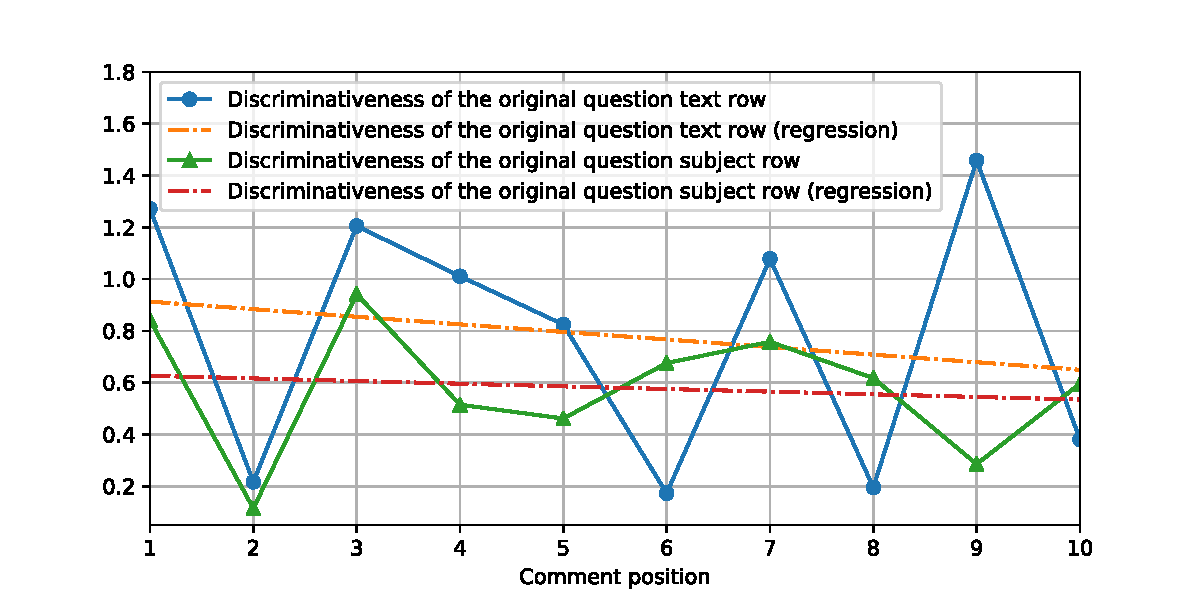
\includegraphics[trim={1.8cm 0.3cm 1.9cm 1.2cm}, scale=0.75]{figs/quality-evaluation-3}
\caption[The discriminativeness of the individual elements of a matrix
$\mathbf{M}_{uv}$ expressed by the absolute values of the machine-learned
coefficients $\bm{\beta}$]{%
  The discriminativeness of the individual elements of a matrix
  $\mathbf{M}_{uv}$\index{.muv@$\mathbf{M}_{uv}$} expressed by the absolute values
  of the machine-learned coefficients $\bm{\beta}$\index{.b@$\bm\beta$ (classifier
  coefficients)}. The discriminativeness of the original question text row
  corresponds to $|\beta_{i+2}|,i=1,2.\ldots,10$, and the discriminativeness of
  the original question subject row corresponds to
  $|\beta_{i+14}|,i=1,2,\ldots,10$.}
  \label{fig:segmentation-quality-evaluation-3}
\end{figure}

These discoveries led us to design and evaluate the
$\wavg_{\textrm{Godwin}}$\index{.wavgGodwin@$\wavg_{\textrm{Godwin}}$|emph}
operator, which assigns a weight proportional to $i^{-1}$ to a nugget\index{nugget} at
position~$i$ in accordance to \term{Zipf's law}\index{Zipf's law}. This
decreases the effect of comments that are likely to be irrelevant. Under the
hypothesis that only relevant comments contain (with a higher chance than
random) important terms that describe the meaning of a document, this weighting
scheme pays attention to scores between those nuggets\index{nugget} that are likely to
contain important terms.

Since weighting terms is conceptually and computationally simpler than
segmentation and result aggregation, I will experimentally verify that the
segmentation is meaningful and that the relevance loss occurs at nugget\index{nugget}
boundaries rather than at term boundaries. For that reason, I designed the
\term{Godwin} term weighting method\index{Godwin!term
weighting|emph}\index{Godwin!operator|see{$\wavg_{\textrm{Godwin}}$}} for the
standard model\index{standard model} scoring function.
For each term $t$ at positions $i_1,i_2,\ldots,i_n$ in a nugget, the method
assigns a weight proportional to $\sum_{j=1}^n i_j^{-1}$ to the
supplementary weight vector element~$e_t$ described in
section~\ref{sec:segmentation-scoring-function}. It is easy to show that, given
the right choice of term frequency factor (\texttt{t}\index{.t@\texttt{t}} in
table~\ref{tab:segmentation-smart}) and vector length normalization factor
(\texttt{n}\index{.n@\texttt{n}} in table~\ref{tab:segmentation-smart}), the
standard model scoring function produces the same ordering on unsegmented
threads as the aggregate scoring function defined in terms of the
$\ominus=\wavg_{\textrm{Godwin}},
\omid=\wavg_{\textrm{length}}$\index{.wavgGodwin@$\wavg_{\textrm{Godwin}}$}
\index{.ominus@$\ominus $}\index{.omid@$\kern .2ex\omid $}
\index{.wavglength@$\wavg _{\textrm  {length}}$} operators would on threads
segmented to one nugget\index{nugget} per a token (see
figure~\ref{fig:segmentation-weighting}).

\begin{figure}[tb]
\centering
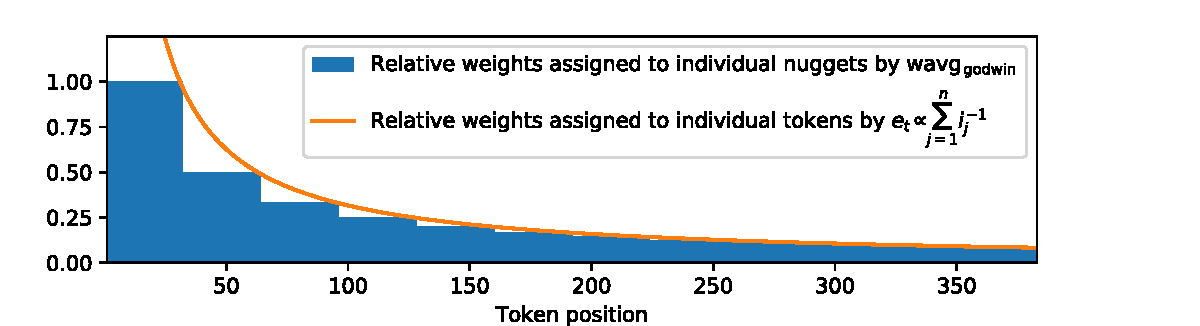
\includegraphics[trim={0.8cm 0.0cm 2.8cm 0.5cm}, scale=0.75]{figs/quality-evaluation-4}
\caption[The relative weights assigned to the individual columns of a matrix
$\mathbf{M}_{uv}$ by the $\wavg_{\textrm{Godwin}}$ operator]{%
  The relative weights assigned to the individual columns of a matrix
  $\mathbf{M}_{uv}$\index{.muv@$\mathbf{M}_{uv}$} by the $\wavg_{\textrm{Godwin}}$ operator plotted along the
  relative weights assigned to the individual tokens by the Godwin term
  weighting\index{Godwin!term weighting} method. The figure assumes the mean
  number of tokens per a thread in the subtask~A unannotated datasets
  (383~tokens), and uniform nugget length in tokens.}
\label{fig:segmentation-weighting}
\end{figure}

\iffalse
\subsubsection{Mutual Information}
\todo{VN: Add the the frequency of 10 terms with the highest ML on the subtask~A
  train dataset in relevant and in the irrelevant comments to conclude that
  there are no terms that can on their discriminate between relevant and
  irrelevant comments. That is why ML is not included in results.}
\fi

\subsection{Parameter estimation}
Some parameters of the scoring functions described in
section~\ref{sec:segmentation-scoring-function} require careful tuning to each particular
dataset. For the standard model\index{standard model}, this corresponds to the
slope parameter~$s$\index{.s@$s$},
which is used by the normalization factors \texttt{u} and \texttt{b} from
table~\ref{tab:segmentation-smart} as a part of pivoted document
normalization~\cite{singhaletal95}. For Okapi \abbr{BM}25\index{Okapi
\abbr{BM}25}, this corresponds to the parameters $k_1,k_3,$ and~$b$.%
\index{.k1@$k_1$}\index{.k3@$k_3$}\index{.b@$b$} Apart from
the scoring functions, the parameter~$l$\index{.l@$l$} of the
BestSentence$_l$\index{.bestsentence@BestSentence${}_l$} nugget
filtering method introduced in section~\ref{sec:segmentation-nugget-filtering}
also requires tuning.

To find the optimum values of $s$\index{.s@$s$}, we initially set $s=0.3$ as
suggested by \textcite{singhaletal95}. By evaluating all the considered
configurations against the subtask~B dev dataset, we obtained the top six
configurations using the normalization factors \texttt{u}\index{.u@\texttt  {u}}
and \texttt{b}\index{.b@\texttt  {b}}, and taking either the unsegmented, machine
learning, or hand-crafted operator approach to result aggregation. I then ran
a grid search to find the values of $s$ in the interval $s\in[0,1]$ maximizing
the performance of these eight configurations.
Figure~\ref{fig:segmentation-slope-optimization} plots the achieved \abbr{MAP}
scores against the choices of parameter~$s$.

\begin{figure}[tb]
\centering%
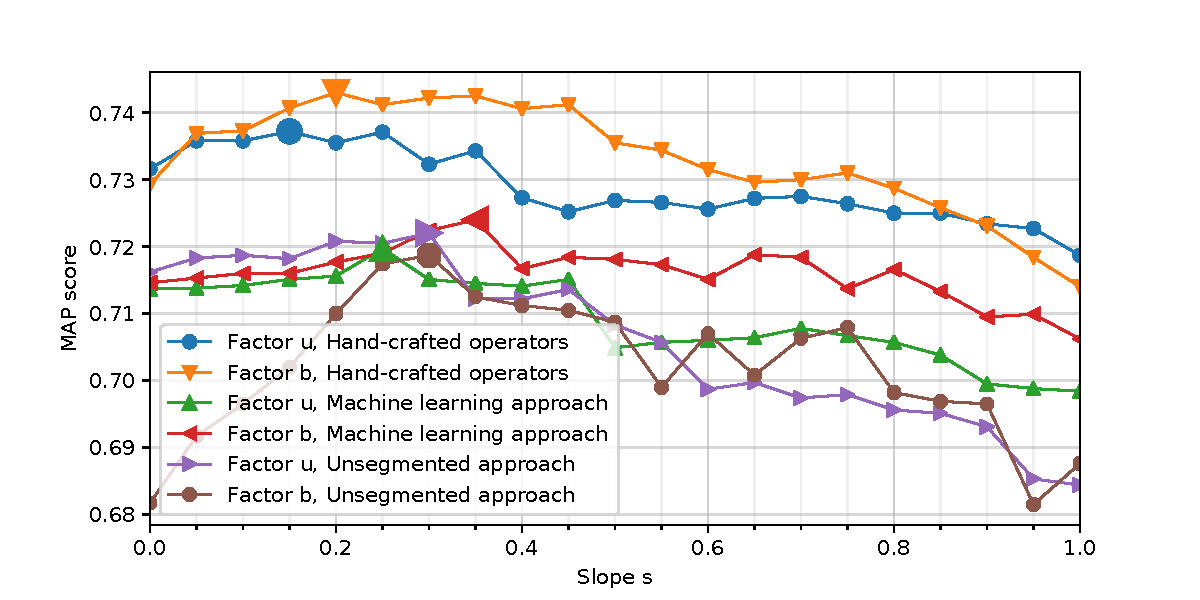
\includegraphics[trim={1.2cm 0.2cm 1.9cm 1.2cm}, scale=0.69]{figs/tfidf}
\caption[The \abbr{MAP} scores achieved with the pivoted normalization factors
\texttt{u} and \texttt{b} for the various choices of the slope parameter~$s$]{%
  The \abbr{MAP} scores achieved with the pivoted normalization factors
  \texttt{u}\index{.u@\texttt{u}} and \texttt{b}\index{.b@\texttt{b}} for the
  various choices of the slope parameter~$s$\index{.s@$s$}.\iffalse Notice that the
  pivoted document normalization is most impactful with the unsegmented
  approach, where the document length varies the most.\fi}
\label{fig:segmentation-slope-optimization}
\end{figure}

To find the optimum values of $k_1,k_3,$ and~$b$\index{.k1@$k_1$}%
\index{.k3@$k_3$}\index{.b@$b$}, we initially set $k_1=1.2,k_3=1000,$
and~$b=0.75$ as suggested by \textcite{singhal01}.
Using the same procedure as above in the intervals $k_1\in[1,2],
k_3\in[0,1000],$ and $b\in[0,1]$, we found the optimal
parameters to be $k_1=2,k_3=950,$ and $b=0$ for the unsegmented approach,
$k_1=2,k_3=0,$ and $b=0.80$ for the machine learning approach, and
$k_1=1.2,k_3=0,$ and $b=0.75$ for the hand-crafted operator approach to result
aggregation.

To find the optimum values of $l$\index{.l@$l$}, we took the
best-performing configuration using the hand-crafted operator approach on the
subtask~B dev dataset (note that
BestSentence$_l$\index{.bestsentence@BestSentence${}_l$} is a nugget
filtering\index{nugget!filtering} method producing a variable number of
nuggets, which makes it unsuitable for both the unsegmented and the machine
learning approach). I then ran a grid search to find the values of $l$ in the
interval $l\in[0,5]$ maximizing the performance of this configuration. Although
\textcite{kolczetal00} suggest the value of $l=3$ in the context of news
articles, the typical question subjects and nuggets\index{nugget} in our
datasets are shorter than the typical news article titles and paragraphs. As a
result, we found more success with less aggressive filtering using $l=0,$ and
$l=1$.

\section{Results}
\label{sec:segmentation-results}
All the 44,496 configurations (twelve~nugget filtering\index{nugget!filtering}
methods, 17~preselected standard model\index{standard model} weighting
schemes, four~supplementary word vectors, four~sets of
Okapi~\abbr{BM}25 parameters\index{Okapi \abbr{BM}25}, 36~pairs of handcrafted
operators, and two~aggregate scoring functions
$S'_{\textrm{query-first}}$ and $S'_{\textrm{result-first}}$) were evaluated on the
\index{.s'queryfirst@$S'_{\text  {query-first}}$}
\index{.s'resultfirst@$S'_{\text  {result-first}}$}
SemEval-2016 and 2017 task~3 subtask~B \abbr{QA} datasets.
Tables~\ref{tab:segmentation-results-2016} and \ref{tab:segmentation-results-2017} show the results.
Although various configurations achieved outstanding \abbr{MAP} scores on one
or the other dataset, only the \term{primary} configuration (highlighted in
bold and italics) consistently achieved scores higher than the winning SemEval
submissions. This configuration uses the \texttt{bfx.nfx} standard model\index{standard model}
weighting scheme suggested by \textcite{ml:SaltonBuckley1988}
for short and homogeneous documents, and the
$\ominus=\wavg_{\textrm{Godwin}}$\index{.wavgGodwin@$\wavg_{\textrm{Godwin}}$}%
\index{.ominus@$\ominus $} handcrafted operator developed in
section~\ref{sec:segmentation-dataset-analysis}.  This shows that the
$\wavg_{\textrm{Godwin}}$ operator is well-suited to our datasets and hopefully
to \abbr{QA} datasets in general.

Several \term{contrastive} configurations that use the unsegmented approach to
result aggregation were derived from the primary configuration. The contrastive
configuration using the Godwin term weighting\index{Godwin!term weighting}
(denoted \term{\texttt{bfx.nfx}, Godwin} in the tables) performed consistently
worse than the primary configuration, which shows that the segmentation to
nuggets\index{nugget} is meaningful and cannot be replaced with term weighting.

\begin{sidewaystable}[p]
\pagestyle{empty}
\centering
\begin{liningfigs}
\begin{tabular}{lllllll}
Rslt. aggregation &
  Nggt. filtering &
  Scoring function &
  Operator $\ominus$\index{.ominus@$\ominus $} &
  Operator $\omid$\index{.omid@$\kern .2ex\omid $} &
  $S'$\index{.s'@$S'$} &
  \abbr{MAP}\index{map@\abbr {MAP}} \\ \toprule
Handcrafted &
  FirstTwoPara\index{.firsttwopara@FirstTwoPara} &
  \texttt{dpc.ann} &
  $\max$ &
  $\wavg_{\textrm{length}}$\index{.wavglength@$\wavg _{\textrm  {length}}$} &
  $S'_{\textrm{query-first}}$ &
  77.25 \\
Handcrafted &
  --- &
  \texttt{bfx.nfx} &
  $\wavg_{\textrm{Godwin}}$ &
  $\wavg_{\textrm{Godwin}}$ &
  $S'_{\textrm{result-first}}$ &
  \index{.s'resultfirst@$S'_{\text  {result-first}}$}
  77.23 \\
Handcrafted &
  FirstTwoPara &
  \texttt{dpc.ann} &
  $\max$ &
  $\wavg_{\textrm{length}}$ &
  $S'_{\textrm{result-first}}$ &
  77.09 \\
Handcrafted &
  FirstTwoPara &
  \texttt{nfc.dfc}, Murata$_{\textrm B}$\index{.muratab@Murata$_{\textrm B}$} &
  $\avg$ &
  $\min$ &
  $S'_{\textrm{result-first}}$ &
  77.00 \\
Handcrafted &
  FirstTwoPara &
  \texttt{Lpc.ann} &
  $\wavg_{\textrm{length}}$ &
  $\max$ &
  $S'_{\textrm{query-first}}$ &
\index{.s'queryfirst@$S'_{\text  {query-first}}$}
  76.96 \\
\itshape\bfseries Handcrafted &
  --- &
  \bfseries\itshape\texttt{bfx.nfx} &
  \bfseries$\textit{wavg}_{\textit{Godwin}}$\index{.wavgGodwin@$\wavg_{\textrm{Godwin}}$} &
  \bfseries$\textit{wavg}_{\textit{length}}$ &
  \bfseries$\bm S'_{\textit{result-first}}$ &
  \bfseries\itshape76.77 \\
\multicolumn{4}{l}{\bfseries SemEval-2016 task~3 subtask~B winner (\abbr{UH-PRHLT}-primary)} &
  --- &
  --- &
  \bfseries76.70 \\
Unsegmented &
  FirstTwoPara &
  \texttt{Lfb.bfc}, Murata$_{\textrm B}$\index{.muratab@Murata$_{\textrm B}$} &
  --- &
  --- &
  --- &
  76.58 \\
Machine learning &
  FirstPara\index{.firstpara@FirstPara} &
  \texttt{nfc.lfc} &
  --- &
  --- &
  --- &
  75.63 \\
\itshape Unsegmented &
  \itshape FirstTwoPara &
  \itshape\texttt{bfx.nfx} &
  --- &
  --- &
  --- &
  \itshape75.21 \\
\multicolumn{3}{l}{\bfseries SemEval-2016 task~3 subtask~B \abbr{IR}\index{ir@\protect\abbr{IR}} baseline} &
  --- &
  --- &
  --- &
  \bfseries74.75 \\
\itshape Unsegmented &
  --- &
  \itshape\texttt{bfx.nfx} &
  --- &
  --- &
  --- &
  \itshape73.94 \\
\itshape Unsegmented &
  --- &
  \itshape\texttt{bfx.nfx}, Godwin &
  --- &
  --- &
  --- &
  \itshape70.28 \\
\end{tabular}
\end{liningfigs}
\caption[Results for the top five configurations on the 2016
subtask~B test dataset]{%
  Results for the top five configurations on the 2016
  subtask~B test dataset, the primary configuration (highlighted in bold
  and italics) with its contrastive configurations (highlighted in italics),
  the top unsegmented and machine learning configurations. The
  \abbr{IR} baseline and the winning submission are highlighted in
  bold.}
\label{tab:segmentation-results-2016}
\end{sidewaystable}

\begin{sidewaystable}[p]
\centering
\begin{liningfigs}
\begin{tabular}{lllllll}
Rslt. aggregation &
  Nggt. filtering &
  Scoring function &
  Operator $\ominus$\index{.ominus@$\ominus $} &
  Operator $\omid$\index{.omid@$\kern .2ex\omid $} &
  $S'$\index{.s'@$S'$} &
  \abbr{MAP}\index{map@\abbr {MAP}} \\ \toprule
Handcrafted &
  BestSentence$_0$\index{.bestsentence@BestSentence${}_l$} &
  Okapi \abbr{BM}25 &
  $\avg$ &
  $\max$ &
  $S'_{\textrm{result-first}}$ &
  49.20 \\
Handcrafted &
  BestSentence$_0$ &
  Okapi \abbr{BM}25 &
  $\avg$ &
  $\wavg_{\textrm{Godwin}}$\index{.wavgGodwin@$\wavg_{\textrm{Godwin}}$} &
  $S'_{\textrm{result-first}}$ &
  \index{.s'resultfirst@$S'_{\text  {result-first}}$}
  48.87 \\
Handcrafted &
  BestSentence$_0$ &
  Okapi \abbr{BM}25 &
  $\avg$ &
  $\max$ &
  $S'_{\textrm{query-first}}$ &
  \index{.s'queryfirst@$S'_{\text  {query-first}}$}
  48.79 \\
Handcrafted &
  BestSentence$_0$ &
  \texttt{bfx.nfx}, Murata$_{\textrm A}$\index{.murataa@Murata$_{\textrm A}$} &
  $\max$ &
  $\wavg_{\textrm{Godwin}}$ &
  $S'_{\textrm{result-first}}$ &
  48.76 \\
Handcrafted &
  BestSentence$_0$ &
  Okapi \abbr{BM}25 &
  $\avg$ &
  $\wavg_{\textrm{Godwin}}$ &
  $S'_{\textrm{result-first}}$ &
  48.76 \\
Unsegmented &
  FirstTwoPara\index{.firsttwopara@FirstTwoPara} &
  \texttt{Lpu.Lpc}, Murata$_{\textrm A}$\index{.murataa@Murata$_{\textrm A}$} &
  --- &
  --- &
  --- &
  48.75 \\
\bfseries\itshape Handcrafted &
  --- &
  \bfseries\itshape\texttt{bfx.nfx} &
  \bfseries$\textit{wavg}_{\textit{Godwin}}$ &
  \bfseries$\textit{wavg}_{\textit{length}}$ &
  \bfseries$\bm S'_{\textit{result-first}}$ &
  \bfseries\itshape47.45 \\
\multicolumn{4}{l}{\bfseries SemEval-2017 task~3 subtask~B winner (SimBow-primary)} &
  --- &
  --- &
  \bfseries47.22 \\
Machine learning &
  FirstTwoPara &
  \texttt{bfx.nfx} &
  --- &
  --- &
  --- &
  46.90 \\
\itshape Unsegmented &
  \itshape FirstTwoPara &
  \itshape\texttt{bfx.nfx} &
  --- &
  --- &
  --- &
  \itshape44.67 \\
\multicolumn{3}{l}{\bfseries SemEval-2017 task~3 subtask~B \abbr{IR}\index{ir@\protect\abbr{IR}} baseline} &
  --- &
  --- &
  --- &
  \bfseries41.85 \\
\itshape Unsegmented &
  --- &
  \itshape\texttt{bfx.nfx}, Godwin &
  --- &
  --- &
  --- &
  \itshape37.18 \\
  %this is baseline, right? any way to tell it to the reader?
\itshape Unsegmented &
  --- &
  \itshape\texttt{bfx.nfx} &
  --- &
  --- &
  --- &
  \itshape36.82 \\
\end{tabular}
\end{liningfigs}
\caption[Results for the top five configurations on the 2017
subtask~B test dataset]{%
  Results for the top five configurations on the 2017
  subtask~B test dataset, the primary configuration (highlighted in bold
  and italics) with its contrastive configurations (highlighted in italics),
  the top unsegmented and machine learning configurations. The
  \abbr{IR} baseline and the winning submission are highlighted in
  bold.}
\label{tab:segmentation-results-2017}
\end{sidewaystable}

The two remaining contrastive configurations using no nugget filtering and the
FirstTwoPara\index{.firsttwopara@FirstTwoPara} nugget
filtering\index{nugget!filtering} show that without segmentation, the standard
model\index{standard model} is unable to cope with the outlier terms introduced by irrelevant
comments. Removing all nuggets\index{nugget} other than the question subject and text
improves the \abbr{MAP} score, but at the cost of losing important terms. The
primary configuration achieves the highest \abbr{MAP} score by properly
weighting the individual nuggets\index{nugget}.

\iffalse
\todo{VN: Significance tests a Density of MAP figures, see:
  \url{https://km.aifb.kit.edu/ws/semsearch10/Files/bm25f.pdf\#page=7}}

\subsubsection{Qualitative Analysis}
\label{sec:segmentation-qualitative-analysis}
\todo{VN: %
  \url{https://gitlab.fi.muni.cz/xnovot32/segmentation-experiments/blob/old-quality-evaluation/quality\_evaluation/quality\_evaluation.ipynb},
  although it would be ideal to update the code as well as the tested configuration
  before publishing.}
\fi

\section{Conclusion and future work}
\label{sec:segmentation-conclusion}
Segmentation matters and so does careful weighting. By combining both, I was
able to achieve state-of-the-art results on the SemEval-2016 and 2017 task~3
subtask~B \abbr{QA} datasets using the standard bag-of-words vector space
model\index{standard model} without semantic modelling. Our method can be
readily implemented into existing inverted-index-based search engines.

\ifreview
Rygl\etal~\cite{rygletal17} have recently shown
\else
We have recently shown~\cite{rygletal17}
\fi
that arbitrary vector space models (e.g.\ \abbr{LSA}\index{LSA@\abbr{LSA}},
\abbr{LDA}, Doc2vec\index{Doc2vec}, \ldots\kern-.2ex) can be used to represent documents
in inverted-index-based search engines.
Evaluating how the concepts of segmentation and result aggregation interact
with semantic models that are not based on a bag-of-words representation
is an intriguing direction for future research.

I have shown \ifthesis in section~\ref{sec:segmentation-dataset-analysis} \fi that there is a
statistically significant relationship between the position of a comment and
its relevance in the SemEval-2016 and 2017 subtask~A datasets. Investigating whether such a relationship exists in other \abbr{QA} datasets (and other datasets in
general) will provide us with new insights to the dynamics of online discourse and
lead to more effective retrieval systems.

\iffalse
As shown in section~\ref{sec:segmentation-dataset-analysis}, there is a statistically
significant relationship between the position of a comment and its relevance
in the SemEval-2016 and 2017 subtask~A datasets. This may 
\todo{VN: Segmentation does matter, but depends on data (Godwin weighting for QA
dataset).  Good term weighting does matter, too.  Taking care of both, we gain
best results on Semeval data even with the standard bag-of-words vector space
representations.}
\todo{VN: We have recently shown how arbitrary vector-space models, such as the
  bag-of-topics LSA and LDA vector spaces, can be represented in
  inverted-index-based search engines:
  \url{http://www.aclweb.org/anthology/W17-2611} How would our system work
  on general vector space models?}
\todo{VN: Would the detection of phrases help our model? Initial testing suggests
  that it would not:
  \url{https://gitlab.fi.muni.cz/xnovot32/segmentation-experiments/wikis/report-2017-10-11}
  but we did not do detection on sequences to filter out incorrectly-detected
  phrases and neither did we try to include both the original phrase and its
  constituents into the document vector. (Perhaps show a table of the top-ranking
  phrase candidates.)}
\todo{VN: How well do our methods generalize to other datasets?}
\todo{VN: The machine learning segmented approach can be generalized to
  documents with a variable number of nuggets by normalizing the dimensions of
  the pairwise nugget similarity matrix, or by treating the matrix as an image
  and the relevance prediction problem as an image classification problem. No
  experiments were conducted to test the performance of this model.}
\todo{VN: How well do our methods generalize to other datasets?}
\todo{VN: (Kołcz\etal 2000, sec. 4) suggests the use of mutual information for term weighting when classification data is available}
\fi
% 
% What else? tokens -> moving to dense latent semantic space, space for even further improvements.

%\nocite{rehurek_lrec,nlp:LSA1990}

\chapter{Modeling Synonymy}
\label{chap:synonymy}
Standard text retrieval methods underestimate the semantic similarity between
documents that use synonymous terms. Latent semantic indexing (\abbr{LSA}\index{LSA@\abbr{LSA}}) tackles the
problem by clustering frequently co-occuring terms at the cost of the periodical
reindexing of dynamic document collections and the suboptimality of
co-occurences\index{term co-occurence} as a measure of synonymy. In this
chapter, I develop a term similarity model that suffers neither of these
flaws. I analyze the associated computational complexity, show how the model
can be implemented into existing \abbr{IR}\index{ir@\abbr {IR}} systems, and
evaluate its performance on the semantic text similarity task.

\section{Introduction}
\label{sec:similarity-introduction}
The standard bag-of-words vector space model~\cite{ir:Salton1975}\index{standard model}
represents documents as vectors in high-dimensional real vector spaces.
The documents are traditionally expressed in a basis where each basis vector
corresponds to a single term, and each coordinate corresponds to the frequency
of a term in our document. Consider the documents
\begin{align*}
  d_1 &=\text{``When Antony found Julius Caesar dead''}, \text{and}\index{.d1@$d_1$} \\
  d_2 &=\text{``I did enact Julius Caesar: I was killed i' the Capitol''}\index{.d2@$d_2$}
\end{align*}
represented in a basis $\{\bm\alpha_i\}_{i=1}^{14}$\index{.a@$\bm\alpha$|emph} of
$\mathbb R^{14}$, where the basis vectors corresponds
to the following terms: when, Anthony, found, Julius, Caesar, dead, I, did, enact, was,
killed, i', the, Capitol. Then the corresponding vectors $\mathbf v_1$ and
$\mathbf v_2$ would have the following coordinates in basis $\bm\alpha$:
\begin{align*}
  \mathbf v_1^{\bm\alpha} &= [1\:1\:1\:1\:1\:1\:0\:0\:0\:0\:0\:0\:0\:0]\tran, \text{and} \\
  \mathbf v_2^{\bm\alpha} &= [0\:0\:0\:1\:1\:0\:1\:1\:1\:1\:1\:1\:1\:1]\tran.
\end{align*}

Since rare words are more important for describing a document than frequent
words, we generally do not assume that $\bm\alpha$\index{.a@$\bm\alpha$} is orthonormal, and we
cast the coordinates into an orthonormal basis $\bm\delta$\index{.d@$\bm\delta$}
chosen in such a way that the frequencies of rare words are amplified. However,
the assumption is usually made that $\bm\alpha$ is orthogonal. This has the
practical advantage that we can directly compute the inner product as a measure
of similarity between any two vectors expressed in $\bm\alpha$. Assuming
$\bm\alpha$ is orthonormal, we may take the inner product between the
normalized $\mathbf v_1$ and $\mathbf v_2$ to measure the similarity between
$d_1$ and $d_2$:
\begin{equation*}
  \langle\mathbf v_1/\Vert \mathbf v_1\Vert, \mathbf v_2/\Vert\mathbf
  v_2\Vert\rangle_{\mathbb{R}^{14}} = \Big(\!(\mathbf v_1^{\bm\alpha})\tran \mathbf v_2^{\bm\alpha}\Big) \Big/ \!
  \left(\!\sqrt{\mathbf (\mathbf v_1^{\bm\alpha})\tran \mathbf
  v_1^{\bm\alpha}}\sqrt{\mathbf (\mathbf v_2^{\bm\alpha})\tran \mathbf
  v_2^{\bm\alpha}}\right)\approx0.26.
\end{equation*}
Intuitively, this underestimates the true similarity between $d_1$ and $d_2$.
If we assume $\bm\alpha$\index{.a@$\bm\alpha$} is non-orthonormal, and that the terms Anthony, Julius, and
Caesar are five times more important than the other terms, then we might construct
a diagonal change-of-basis matrix\note{%
The main diagonal of $\mathbf W$ corresponds to the
nugget frequency factor in table~\ref{tab:segmentation-smart}.} $\mathbf W =
(w_{ij})$\index{.w@$\mathbf W$|emph} from $\bm\alpha$ to an orthonormal basis
$\bm\delta$\index{.d@$\bm\delta$}, where
\begin{equation}
  \label{eq:similarity-W}
  w_{ij} = \begin{cases}
    5 & \text{if } i = j, i \in\{\textrm{Anthony}, \textrm{Julius}, \textrm{Caesar}\}, \\
    1 & \text{if } i = j, i \not\in\{\textrm{Anthony}, \textrm{Julius}, \textrm{Caesar}\}, \text{and} \\
    0 & \text{if } i \not= j. \\
  \end{cases}
\end{equation}
Then $\mathbf v_1$ and $\mathbf v_2$ would have the following coordinates in
$\bm\delta$\index{.d@$\bm\delta$}:
\begin{align*}
  \mathbf v_1^{\bm\delta} &= \mathbf W \mathbf v_1^{\bm\alpha} = [1\:5\:1\:5\:5\:1\:0\:0\:0\:0\:0\:0\:0\:0]\tran, \text{and} \\
  \mathbf v_2^{\bm\delta} &= \mathbf W \mathbf v_2^{\bm\alpha} = [0\:0\:0\:5\:5\:0\:1\:1\:1\:1\:1\:1\:1\:1]\tran,
\end{align*}
and our inner product would change to
\begin{multline*}
  \langle\mathbf v_1/\Vert \mathbf v_1\Vert, \mathbf v_2/\Vert\mathbf v_2\Vert\rangle_{\mathbb{R}^{14}}
  = \Big(\!(\mathbf v_1^{\bm\delta})\tran \mathbf v_2^{\bm\delta}\Big) \Big/\!
    \left(\!\!\sqrt{\mathbf (\mathbf v_1^{\bm\delta})\tran \mathbf
    v_1^{\bm\delta}}\sqrt{\mathbf (\mathbf v_2^{\bm\delta})\tran \mathbf
    v_2^{\bm\delta}}\right) ={}\\
  {}= \Big(\!(\mathbf W\mathbf v_1^{\bm\alpha})\tran (\mathbf W\mathbf v_2^{\bm\alpha})\!\Big) \Big/\!
    \left(\!\!\sqrt{\mathbf (\mathbf W\mathbf v_1^{\bm\alpha})\tran (\mathbf W\mathbf
    v_1^{\bm\alpha})}\sqrt{(\mathbf W\mathbf v_2^{\bm\alpha})\tran (\mathbf W\mathbf
    v_2^{\bm\alpha})}\right)\approx0.89.
\end{multline*}
Intuitively, this comes closer to the true similarity between $d_1$ and $d_2$.

Although the assumption that $\bm\alpha$\index{.a@$\bm\alpha$} is orthogonal has been an inherent
part of the standard model since its inception, it makes modeling synonymy
difficult. The terms dead and killed contribute nothing to the inner product of
$\mathbf v_1$ and $\mathbf v_2$ despite the clear synonymy, since we assume
$\langle \bm\alpha_{\text{dead}}, \bm\alpha_{\text{killed}}\rangle_{\mathbb
R^{14}}=0$. In general, the standard model will underestimate the true
similarity between documents that carry the same meaning, but use different
terminology. In this \ifthesis chapter\else work\fi, I extend the standard
model\index{standard model!extended} to non-orthogonal bases and experimentally
evaluate several properties of the extended model.\note{%
\ifreview
A link to the research data will be disclosed in the camera-ready
version of the paper.
\else
\url{https://github.com/witiko-masters-thesis/similarity}
\fi}

The chapter is structured as follows: In section~\ref{sec:similarity-relwork}, I
review the previous research in the area of modeling synonymy in the standard
model. I provide a mathematical definition of the extended standard model and
place upper asymptotic complexity bounds on computing the similarity between two
documents in sections~\ref{sec:similarity-model} and
\ref{sec:similarity-complexity}. I then develop several term similarity matrices
for the extended model in section~\ref{sec:similarity-measures}. In
section~\ref{sec:similarity-system}, I consider several approaches to
implementing the extension into existing tools. I describe the experiments that
I carried out on the dataset in
section~\ref{sec:similarity-experimental-setup}; the results are presented in
section~\ref{sec:similarity-results}. I conclude in
section~\ref{sec:similarity-conclusion} by summarizing the results, and
suggesting future work.

\section{Related work}
\label{sec:similarity-relwork}
The notion of modeling document similarity using a non-orthogonal coordinate
system was perhaps first explored by \textcite{sidorov2014soft} in the context
of entrance exam question answering, where the basis vectors did not correspond
directly to terms, but rather to $n$-grams constructed by
following paths in syntactic trees. They derive the inner product between two
basis vectors from the edit distance\index{edit distance} between the
corresponding $n$-grams.

A notable contribution of \textcite{sidorov2014soft} is a formula for computing
the inner product between two vectors expressed in a non-orthogonal basis
without performing an explicit change of basis. The formula was termed \term{soft
cosine similarity}\index{cosine similarity!soft}, perhaps because the
inner product between two normalized vectors corresponds to the cosine of the
angle between the vectors (often referred to as the \term{cosine
similarity}\index{cosine similarity|emph}), and the nonzero inner product
between basis vectors induces soft clustering of the individual $n$-grams.
Notably, they also develop two algorithms for casting the coordinates to an
orthonormal basis. In section~\ref{sec:similarity-complexity}, I show that one
of the algorithms is time-suboptimal.

\textcite{charletdamnati17} won SemEval-2017 task~3
subtask~B~\cite{nakov2017semeval} by training a supervised classifier using
soft cosine similarity between every possible combination of subparts of an
original question and a thread. Unlike \textcite{sidorov2014soft},
\textcite{charletdamnati17} already use basis vectors that correspond to terms.
Notably, they derive the inner product between two basis vectors from the inner
product between the corresponding terms embedded in a
Word2vec\index{Word2vec|emph}~\cite{mikolov2013efficient}
space. I further develop this notion in section~\ref{sec:similarity-measures}.

\section{Extended model}
\label{sec:similarity-model}
In this section, I state a formal definition of the extended standard
model\index{standard model!extended} and describe key properties of the model.

Let $\mathbb R^n$\index{.n@$n$|emph} be the finite inner-product space over
$\mathbb R$ from which we draw our feature vectors. Let
$\langle\cdot,\cdot\rangle_{\mathbb R^n}$ be the bilinear inner product on
$\mathbb R^n$ and $\{\bm{\beta}_i\}_{i = 1}^n$\index{.b@$\bm\beta$ (basis)|emph}
the basis in which our feature vectors are expressed. Assume that
$\bm{\beta}$\index{.b@$\bm\beta$ (basis)} is non-orthogonal, i.e. that $\exists i,
j: i\not=j, \langle \bm{\beta}_i,
\bm{\beta}_j\rangle_{\mathbb R^n} \not= 0$. Let $\mathbf W=(w_{ij})$\index{.w@$\mathbf
W$} be a diagonal change-of-basis matrix from $\bm\beta$ to a non-orthogonal
normalized basis $\{\bm{\gamma}_i\}_{i = 1}^n$\index{.c@$\bm\gamma$|emph} of
$\mathbb R^n$, i.e. $\forall i, j: \langle \bm{\gamma}_i,
\bm{\gamma}_j\rangle_{\mathbb R^n}\in[-1, 1], \langle \bm{\gamma}_i,
\bm{\gamma}_i\rangle_{\mathbb R^n}=1$.  Let $\mathbf S=(s_{ij})$\index{.s@$\mathbf
S$|emph}, where $s_{ij} = \langle \bm{\gamma}_i, \bm{\gamma}_j\rangle_{\mathbb
R^n}$. Since $\mathbf S$ is a matrix of inner products between linearly
independent vectors, it is Gramian\index{matrix!Gramian} and therefore positive
definite\index{matrix!positive definite} and Hermitian%
\index{matrix!Hermitian}. Let $\mathbf E$\index{.e@$\mathbf E$|emph} denote the
change-of-basis matrix from $\bm\gamma$\index{.c@$\bm\gamma$} to some orthonormal
basis $\bm\delta$\index{.d@$\bm\delta$|emph} of $\mathbb R^n$.

Take any two feature vectors $\mathbf x, \mathbf y\in\mathbb R^n$ and let
$\mathbf x^{\bm{\beta}}, \mathbf y^{\bm{\beta}}$ denote the coordinates of
$\mathbf x$ and $\mathbf y$ in the basis $\bm\beta$\index{.b@$\bm\beta$ (basis)}.
By expressing $\mathbf x$ and $\mathbf y$ in the orthonormal basis
$\bm\delta$\index{.d@$\bm\delta$}, we can express the inner product between
$\mathbf x$ and $\mathbf y$ in terms of an algebraic dot product,
i.e.\begin{multline}
  \label{eq:similarity-inner-product}
  \langle\mathbf x, \mathbf y\rangle_{\mathbb R^n}
  = (\mathbf{x}^{\bm\delta})\tran (\mathbf{y}^{\bm\delta})
  = (\mathbf{Ex}^{\bm\gamma})\tran (\mathbf{Ey}^{\bm\gamma})
  = (\mathbf{EWx}^{\bm\beta})\tran (\mathbf{EWy}^{\bm\beta}) ={} \\
  = \left(\sum_{i=1}^n \bm{\beta}_i^{\bm\delta}w_{ii}x_i^{\bm\beta}\right)\left(\sum_{j=1}^n\bm{\beta}_i^{\bm\delta}w_{ii} y_i^{\bm\beta}\right)
  = \sum_{i=1}^n\sum_{j=1}^nw_{ii}x_i^{\bm\beta}w_{jj}y_j^{\bm\beta} \langle\bm\beta_i, \bm\beta_j\rangle_{\mathbb R^n} ={} \\
  = \sum_{i=1}^n\sum_{j=1}^nw_{ii}x_i^{\bm\beta}w_{jj}y_j^{\bm\beta} s_{ij}
  = (\mathbf{Wx}^{\bm\beta})\tran \mathbf S\mathbf{Wy}^{\bm\beta}
  = (\mathbf{x}^{\bm\gamma})\tran \mathbf S\mathbf{y}^{\bm\gamma}
\end{multline}
Therefore we only need to supply a positive-definite\index{matrix!positive
definite} Hermitian matrix\index{matrix!Hermitian} $\mathbf{S}$\index{.s@$\mathbf
S$} and a diagonal matrix $\mathbf W$\index{.w@$\mathbf W$} to compute the inner
product between $\mathbf x$ and $\mathbf y$; computing $\mathbf E$
\index{.e@$\mathbf E$} is unnecessary. I give several examples of such matrices
$\mathbf S$ in section~\ref{sec:similarity-measures}. From here, we can
directly derive the cosine of the angle between $\mathbf x$ and $\mathbf y$,
i.e. the soft cosine similarity\index{cosine similarity!soft} formula
\begin{equation}
\label{eq:similarity-soft-cosine}
\begin{aligned}
  \langle\mathbf x/\Vert\mathbf x\Vert, \mathbf y/\Vert\mathbf y\Vert\rangle_{\mathbb R^n} &= 
  \frac{(\mathbf x^{\bm\gamma})\tran\mathbf S\mathbf y^{\bm\gamma}}{\sqrt{\strut((\mathbf x^{\bm\gamma})\tran\mathbf S\mathbf x^{\bm\gamma}}\sqrt{\strut(\mathbf y^{\bm\gamma})\tran\mathbf S\mathbf y^{\bm\gamma}}} = \\
  &= \frac{(\mathbf{Wx}^{\bm\beta})\tran\mathbf S\mathbf{Wy}^{\bm\beta}}{\sqrt{\strut((\mathbf{Wx}^{\bm\beta})\tran\mathbf S\mathbf{Wx}^{\bm\beta}}\sqrt{\strut(\mathbf{Wy}^{\bm\beta})\tran\mathbf S\mathbf{Wy}^{\bm\beta}}}.
\end{aligned}
\end{equation}

\section{Complexity analysis}
\label{sec:similarity-complexity}
In this section, I place upper worst-case asymptotic complexity bounds on
computing the inner product and on casting vector coordinates to an orthonormal
basis. Unlike previous work, I focus on bases that are mostly orthogonal,
i.e. bases whose corresponding matrices $\mathbf S$\index{.s@$\mathbf S$} are very
sparse outside the main diagonal, and prove lower complexity bounds for such
bases.

Following the notation of \textcite{ml:IntroIR2008}, let
$M_{\max}$\index{.mmax@$M_{\max}$|emph} denote the maximum number of terms in a document,
and let $C$\index{.c@$C$|emph} be the maximum number of nonzero non-diagonal
elements in a row of a matrix $\mathbf S$.

\subsection{Inner product}
\paragraph{Time complexity} First, I show that a time-optimal algorithm
for computing the inner product between two document vectors $\mathbf x$ and
$\mathbf y$ will perform no more than $(C+1)M_{\max}$ steps. To see why,
consider the expression\begin{equation*}
  \sum_{i=1}^n\sum_{j=1}^nw_{ii}x_i^{\bm\beta}w_{jj}y_j^{\bm\beta}
  s_{ij}
\end{equation*} from equation~\ref{eq:similarity-inner-product}. By our
assumption, $x_i^{\bm\beta}$ is nonzero for at most $M_{\max}$ values
of the variable $i$ and for each fixed $i$, $s_{ij}$ is nonzero for at most
$C+1$ values of the variable $j$ (the additional element corresponds to the
ones on the main diagonal of $\mathbf S$\index{.s@$\mathbf S$}). By using an
appropriate data structure to represent the vectors $\mathbf x$ and $\mathbf
y$, e.g. lists of nonzero coordinates in the basis $\bm\beta$\index{.b@$\bm\beta$ (basis)}, the matrix
$\mathbf W$\index{.w@$\mathbf W$}, e.g. an array corresponding to the main
diagonal of $\mathbf W$\index{.w@$\mathbf W$}, and the matrix $\mathbf
S$\index{.s@$\mathbf S$}, e.g. an array of rows represented as a list of nonzero
non-diagonal elements, a time-optimal algorithm will perform at most
$(C+1)M_{\max}$ steps.

\paragraph{Space complexity} Next, I will show that a space-optimal algorithm
for computing the inner product between two document vectors $\mathbf x$ and
$\mathbf y$ will occupy no more than $2M_{\max}+(n+1)C$ units of space, where
$n$\index{.n@$n$} is
the number of basis vectors in the bases $\bm\beta,$\index{.b@$\bm\beta$ (basis)}
$\bm\gamma,$\index{.c@$\bm\gamma$} and $\bm\delta$\index{.d@$\bm\delta$}
as well as the number of terms in our vocabulary. To see why, consider the data
structures given above. The lists representing the vectors $\mathbf x$ and
$\mathbf y$ will occupy at most $M_{\max}$ units of space each, the array
representing the matrix $\mathbf W$\index{.w@$\mathbf W$} will occupy $n$ units of
space, and the sparse matrix $\mathbf S$\index{.s@$\mathbf S$} will occupy at most
$nC$ units of space.

Assuming that $M_{\max}$ and $C$ are arbitrary, i.e. at most $n$, we get a
worst-case time and space complexity of $\Theta(n^2)$. According to the
\term{Heaps' law}\index{Heaps' law|emph}, $n^2\approx T$, where
$T$\index{.t@$T$|emph} is the size of the document collection in tokens. Given the
size of today's document collections, which are routinely ``sharded'' between
several computers since they cannot fit into the memory of a single device,
such space complexity is practically intractable outside distributed computing.

Let us instead assume that $M_{\max}$\index{.mmax@$M_{\max}$} is a constant, i.e. that we can
place an upper limit on how large the vocabulary of any single document can be,
e.g. by limiting the maximum length of a document. Let us also assume that we
can build the matrix $\mathbf S$ in such a way that $C$ is a constant, which
will be the topic of section~\ref{sec:similarity-measures}. Under these
assumptions, the worst-case time complexity of computing the inner product
is $\Theta(1)$ and the worst-case space complexity is $\Theta(n)$.

\subsection{Orthonormalization}
\label{sec:similarity-complexity-orthonormalization}
One way to cast the coordinates of a vector from the basis
$\bm\beta$\index{.b@$\bm\beta$ (basis)} to an orthonormal basis is to compute the
change-of-basis matrix $\mathbf E$\index{.e@$\mathbf E$}, since for any document
vector $\mathbf x$,
\begin{equation*}
  \mathbf x^{\bm\delta} = \mathbf E\mathbf x^{\bm\gamma} = \mathbf E\mathbf W\mathbf x^{\bm\beta}.
\end{equation*}
For ease of reference, I will use $\Phi_1(\mathbf
x^{\bm\beta})$\index{.v1@$\Phi_1$|emph} to denote $\mathbf E\mathbf W\mathbf
x^{\bm\beta}$.
Another way to cast the coordinates of a vector from the basis $\bm\beta$\index{.b@$\bm\beta$ (basis)}
to an orthonormal basis is to express the vector in an orthonormal basis
$\bm\delta'$\index{.d@$\bm\delta'$|emph} of $\mathbb R^{n^2}\!\!$. As shown by
\textcite[sec.~2.4]{sidorov2014soft}, for any document vectors $\mathbf x,
\mathbf y,$\begin{multline}
  \label{eq:similarity-Phi2}
  \langle\mathbf x,\mathbf y\rangle_{\mathbb R^n} = \langle\mathbf x',\mathbf y'\rangle_{\mathbb R^{n^2}},\text{ where }
  x_{ij}^{\prime\bm\delta'}=\sqrt{2c_{ij}}\frac{w_{ii}x_i^{\bm\beta}+w_{jj}x_j^{\bm\beta}}2, \\
  y_{ij}^{\prime\bm\delta'}=\sqrt{2c_{ij}}\frac{w_{ii}y_i^{\bm\beta}+w_{jj}y_j^{\bm\beta}}2,\text{ and }
  c_{ij} = \begin{cases}
    \frac{1-\sum_{k\not=i}s_{ik}}2 & \text{if }i = j\text{, and} \\
    s_{ij} & \text{otherwise}.
  \end{cases}
\end{multline}
For ease of reference, I will use $\Phi_2(\mathbf
x^{\bm\beta})$\index{.v2@$\Phi_2$|emph} to denote $\mathbf x'^{\bm\delta'}$.

\paragraph{Time complexity} First, I will show that a time-optimal algorithm
for casting the coordinates of a document vector $\mathbf x$ to an orthonormal
basis will perform no more than $M_{\max}^2$ steps. To see why, consider the
expression\begin{equation*}
  x_{ij}^{\prime\bm\delta'}=\sqrt{2c_{ij}}\frac{w_{ii}x_i^{\bm\beta}+w_{jj}x_j^{\bm\beta}}2
\end{equation*}
that corresponds to a single coordinate of $\Phi_2(\mathbf x^{\bm\beta})$ in
equation~\ref{eq:similarity-Phi2}. By the assumption from the beginning of the
section, $x_i^{\bm\beta}$ and $x_j^{\bm\beta}$ are nonzero for at most
$M_{\max}$\index{.mmax@$M_{\max}$} values of the variables $i$ and $j$. By using an
appropriate data structure to represent $\mathbf x$, e.g. a list of nonzero
coordinates in the basis $\bm\beta$\index{.b@$\bm\beta$ (basis)}, an optimal
algorithm will compute the $M_{\max}^2$ nonzero coordinates of $\mathbf
x'^{\bm\delta'}$ using no more than $M_{\max}^2$ steps.

By the definition of $\mathbf S$\index{.s@$\mathbf S$}, $\mathbf E\mathbf
E\tran=\mathbf S$.
Furthermore, \textcite[sec.~2.5]{sidorov2014soft} show that $\mathbf E$ is
lower-diagonal. Therefore, by the positive-definiteness\index{matrix!positive
definite} and the hermicity\index{matrix!Hermitian} of $\mathbf S$, $\mathbf E$
\index{.e@$\mathbf E$} is uniquely determined by the \term{Cholesky
factorization}\index{Cholesky
factorization} of $\mathbf S$. Using the well-known Cholesky algorithm, we can
compute $\mathbf E$ in $\mathcal O(n^3)$ steps. This improves on the result of
\textcite[sec.~2.5]{sidorov2014soft} who show that $\mathbf E$ can be computed
from $\mathbf S$ in $\mathcal O(n^4)$\index{.n@$n$} steps. For a document vector
$\mathbf x$, a time-optimal algorithm can then compute $\Phi_1(\mathbf
x^{\bm\beta})$\index{.v1@$\Phi_1$} in no more than $M_{\max}n$ steps. To see why,
consider the expression
\begin{equation*}
  \sum_{i=1}^n \bm{\beta}_i^{\bm\delta}w_{ii}x_i^{\bm\beta}
\end{equation*}
that corresponds to $\Phi_1(\mathbf x^{\bm\beta})$ in
equation~\ref{eq:similarity-inner-product}. By our assumption, $x_i^{\bm\beta}$
is nonzero for at most $M_{\max}$ values of the variable $i$.
Assuming nothing about the density of $\mathbf E$, $\bm\beta_i^{\bm\delta}$
has at most $n$ nonzero values for each fixed~$i$.

\paragraph{Space complexity} Next, I will show that a space-optimal algorithm
for casting the coordinates of a document vector $\mathbf x$ to an orthonormal
basis will occupy no more than $M_{\max}^2+M_{\max}(1+C)+n$\index{.mmax@$M_{\max}$}
units of space.  To see why, consider again that $\mathbf x'^{\bm\delta'}$ has
$M_{\max}^2$ nonzero coordinates. By using an appropriate data structure to
represent $\mathbf x'$, e.g. a list of nonzero coordinates in the basis
$\bm\delta'$, the resulting vector will occupy precisely $M_{\max}^2$ units of
space. The list representing the vector $\mathbf x$ will then occupy at most
$M_{\max}$ units of space, the array representing the matrix $\mathbf
W$\index{.w@$\mathbf W$} will occupy $n$ units of space, and the sparse matrix
$\mathbf S$\index{.s@$\mathbf S$} will occupy at most $nC$ units of space.

If we assume again that nothing is known about the density of $\mathbf
E$\index{.e@$\mathbf E$}, then a space-optimal algorithm computing $\mathbf
E$\index{.e@$\mathbf E$} occupies at most $n(C+n)$\index{.n@$n$}\index{.c@$C$} units of
space. To see why, consider that the Cholesky algorithm is computed in-place,
the sparse matrix $\mathbf S$\index{.s@$\mathbf S$} occupies at most $nC$ units of
space and the resulting matrix $\mathbf E$ occupies at most $n^2$ units of
space. For a document vector $\mathbf x$, a space-optimal algorithm computing
$\Phi_1(\mathbf x^{\bm\beta})$\index{.v1@$\Phi_1$} then occupies at most
$n^2+2n$\index{.n@$n$} units of space. To see why, consider that the matrix
$\mathbf E$ will occupy at most $n^2$ units of space, the array representing
the matrix $\mathbf W$\index{.w@$\mathbf W$} will occupy at most $n$ units of
space, and the resulting vector coordinates will occupy at most $n$ units of
space. Notice that although $\Phi_1$\index{.v1@$\Phi_1$} does not lead to an
increase of dimensionality like $\Phi_2$\index{.v2@$\Phi_2$} does, it can instead
lead to an arbitrary increase of density.

Assuming that $M_{\max}$\index{.mmax@$M_{\max}$} is arbitrary, i.e. at most
$n$\index{.n@$n$}, we get a worst-case time and space complexity of $\Theta(n^2)$.
As I argued in the previous section, such space complexity is practically
intractable outside distributed computing. Let us assume again that
$M_{\max}$\index{.mmax@$M_{\max}$} is a constant. Under this assumption, the
worst-case time complexity of computing the inner product is $\Theta(1)$ and
the worst-case space complexity is $\Theta(n)$.

As a remark, note that although we assumed in the above analysis that
nothing is known about the density of $\mathbf E$\index{.e@$\mathbf E$}, this
does not mean that we cannot find a more compact representation of $\mathbf E$.
Given a sparse matrix $\mathbf S$, we can generally find a permutation matrix
$\mathbf P$\index{.p@$\mathbf P$|emph}, such that the Cholesky
factor\index{Cholesky factorization} $\mathbf L$\index{.l@$\mathbf
L$|emph}, where $\mathbf L\mathbf
L\tran=\mathbf P\mathbf S\mathbf P\tran$, is also sparse.  Using basic facts
about matrix transposition, we can derive $\mathbf E=\mathbf P^{-1}\mathbf L$
as follows:
\begin{equation*}
  \mathbf S
  = \mathbf P^{-1}\mathbf L\mathbf L\tran(\mathbf P\tran)^{-1}
  = \mathbf P^{-1}\mathbf L\mathbf L\tran(\mathbf P^{-1})\tran
  = \mathbf E\mathbf E\tran.
\end{equation*}
This allows us to store a permutation matrix $\mathbf P$ and a sparse matrix
$\mathbf L$\index{.l@$\mathbf L$} instead of an arbitrarily dense
matrix $\mathbf E$. However, the existence of such a permutation matrix
$\mathbf P$\index{.p@$\mathbf P$} is only guaranteed for matrices $\mathbf
S$\index{.s@$\mathbf S$} of a specific structure, and even if such a $\mathbf
P$ exists, the problem of finding it is
\textsf{NP}-complete~\cite{yannakakis1981computing}, so we will generally only
find a suboptimal $\mathbf P$.

\section{Similarity matrices}
\label{sec:similarity-measures}
In this section, I construct several matrices $\mathbf S$\index{.s@$\mathbf
S$} that model different facets of term similarity. Although it is possible to
explicitly construct a change-of-basis matrix $\mathbf E$\index{.e@$\mathbf E$},
it is perhaps easier to construct the matrix $\mathbf S$ of inner products
between the basis vectors. Since we assume the basis vectors of basis
$\bm\gamma$\index{.c@$\bm\gamma$} are normalized, this is equivalent to
constructing a matrix $\mathbf S$\index{.s@$\mathbf S$} of cosines of the angles
between the basis vectors.

If we expect to be computing $\mathbf E$\index{.e@$\mathbf E$}
from $\mathbf S$\index{.s@$\mathbf S$},
then we require $\mathbf S$ to be both positive-definite\index{matrix!positive
definite} and Hermitian\index{matrix!Hermitian}.
Hermicity comes down to simple symmetry in $\mathbb{R}^n$ and as such, it is
easily satisfied; all the matrices shown in this section are Hermitian.
One approach to satisfying positive-definiteness is to satisfy a stronger
condition and build a strictly diagonally dominant matrix $\mathbf S$. In the
context of section~\ref{sec:similarity-complexity}, this can be easily
satisfied by placing only $C=1$\index{.c@$C$} nonzero non-diagonal elements into
each row of $\mathbf S$. If a non-diagonal element has precisely the value $-1$
or $1$, and would therefore violate the strict diagonal dominance of $\mathbf
S$, we will retain only the diagonal element for the corresponding row. All the
matrices $\mathbf S$ shown in this section can be sparsified to this form.

If we expect to be computing only the inner product between two normalized
vectors (i.e. the soft cosine similarity\index{cosine similarity!soft}), then
we require only that $\mathbf x\not=\mathbf0\implies\Vert\mathbf
x\Vert\in\mathbb{R}^+$, i.e. that $\mathbf
x\not=\mathbf0\implies(\mathbf{x}^{\bm\gamma})\tran\mathbf S\mathbf x^{\bm\gamma}>0$.
If we required this for any $\mathbf x\in\mathbb R^n$, then this would be
equivalent to the requirement that $\mathbf S$ is positive
definite\index{matrix!positive definite}. However, since we know that the
coordinates $\mathbf x^{\bm\gamma}$ correspond to term frequencies, which are
non-negative, it is sufficient to require that $\mathbf S$ is non-negative as
well, i.e. that $\forall i, j=1,\ldots,n: s_{ij}\geq0$.  Like
hermicity\index{matrix!Hermitian}, this condition is easy to satisfy, and all
the matrices $\mathbf S$ shown in this section are non-negative.  Note that by
using a matrix $\mathbf S$ that is not positive definite\index{matrix!positive
definite}, we are violating the original assumption that
$\bm\gamma$\index{.c@$\bm\gamma$} is a basis. Nevertheless, these matrices may
still be practically useful, as evidenced by their use in the work of
\textcite{charletdamnati17}.

Lastly, if we expect to be computing only the inner product and only between
two non-normalized vectors, then $\mathbf S$\index{.s@$\mathbf S$} can be arbitrary.

\subsection{Spelling}
One facet of term similarity that we might want to model is spelling.
Intuitively, a two document that are identical except for a single misspelled
term should be also considered nearly identical by our model. We may use
edit distance\index{edit distance} to formalize this intuition.
\textcite{charletdamnati17} propose the following measure:\begin{equation}
  s_{ij} = \begin{cases}
    1 & \text{if }i = j\textrm{,} \\
    0 & \text{if }\theta_1\left(1-\frac{\textrm{edit}(i, j)}{\max(b_i, b_j)}\right)^{\theta_2}\leq\theta_3\textrm{, and} \\
    \theta_1\left(1-\frac{\textrm{edit}(i, j)}{\max(b_i, b_j)}\right)^{\theta_2} & \index{.h1@$\theta_1$|emph}\index{.h2@$\theta_2$|emph}\index{.h3@$\theta _3$|emph}\textrm{otherwise,}
  \end{cases}
\end{equation}
where $\textrm{edit}(i, j)$ is the edit distance between the terms
$i$ and $j$, $b_i$\index{.bi@$b_i$} and $b_j$ are the byte lengths of the terms $i$,
and $\bm\theta$ are parameters whose optimal values on the
subtask~B dev dataset are $\theta_1=1.8,\theta_2=5,$ and $\theta_3=0$ according
to the authors. I will refer to the resulting matrix as $\mathbf
S_{\textrm{lev}}$\index{.slev@$\mathbf  S_{\textrm  {lev}}$|emph} for ease of
reference.

Additionally, I introduce a pruning parameter
$\theta_4$\index{.h4@$\theta_4$|emph} and preemptively assign $s_{ij}=0$ to all
terms $i$ and $j$ such that $\max(b_i, b_j) / \min(b_i, b_j) > \theta_4$.
Intuitively, terms with disproportionate lengths are unlikely to be
misspellings of one another, so this initial pruning saves us the time that we
would otherwise spend computing the edit distance between distant terms.  Due
to the time complexity of edit distance, this parameter was not exhaustively
optimized; instead, the value $\theta_4=1.5$\index{.h4@$\theta_4$} was chosen.

In the context of section~\ref{sec:similarity-complexity}, this formula
provides no efficient procedure to sparsity the matrix $\mathbf
S_{\textrm{lev}}$\index{.slev@$\mathbf  S_{\textrm  {lev}}$}. For each term $i$,
we may compute the value $s_{ij}$ for every other term $j$ that survived the
initial pruning and then assign $s_{ij}\leftarrow 0$ for all but the
$C$\index{.c@$C$} highest values of $s_{ij}$. \textcite{charletdamnati17}
reported using only $C=100$\index{.c@$C$} highest values of $s_{ij}$.

\subsection{Synonymy}
Another facet of term similarity is
synonymy. By building a term co-occurence\index{term co-occurence} model of a dataset, we can derive
an unsupervised measure of synonymy by considering terms occuring in similar
contexts “more synonymous” than terms occuring in different contexts.
\textcite{charletdamnati17} propose the following measure:\begin{equation}
  s_{ij} = \begin{cases}
    1 & \text{if }i = j\textrm{,} \\
    0 & \text{if }\langle\mathbf v_i / \Vert\mathbf v_i\Vert, \mathbf v_j / \Vert\mathbf v_j\Vert\rangle_{\mathbb X}\leq\theta_3\textrm{,\,and} \\
    \langle\mathbf v_i / \Vert\mathbf v_i\Vert, \mathbf v_j / \Vert\mathbf v_j\Vert\rangle_{\mathbb X}^{\theta_5}\index{.h3@$\theta _3$}\index{.h5@$\theta_5$|emph}&\textrm{otherwise,}
  \end{cases}
\end{equation}
where $\mathbf v_i, \mathbf v_j\in\mathbb X$ are the embeddings\index{term
embedding} of the terms $i$ and $j$ in the inner-product space $\mathbb X$ produced by
a term embedding\index{term embedding} model such as
Word2vec~\cite{mikolov2013efficient}\index{Word2vec},
GloVe~\cite{pennington2014glove}\index{GloVe|emph}, or
FastText~\cite{bojanowski2016enriching}\index{FastText|emph},
$\langle\cdot,\cdot\rangle_{\mathbb X}$ is the inner product on $\mathbb
X$\index{.x@$\mathbb X$|emph}, and $\bm\theta$ are parameters whose optimal
values on the subtask~B dev dataset are $\theta_3=0,$ and $\theta_5=2$
according to the authors. I will refer to the resulting matrix as $\mathbf
S_{\textrm{rel}}$\index{.srel@$\mathbf  S_{\textrm  {rel}}$|emph} for ease of
reference.

In the context of section~\ref{sec:similarity-complexity}, this formula
provides an opportunity to sparsify $\mathbf
S_{\textrm{rel}}$\index{.srel@$\mathbf  S_{\textrm  {rel}}$} efficiently.
For each term $i$, we assign $s_{ij}\leftarrow 0$ for all but the
$C$\index{.c@$C$} nearest neighbors $\mathbf v_j$ of $\mathbf v_i$ in $\mathbb X$.
\textcite{charletdamnati17} reported retrieving only $C=100$\index{.c@$C$}
nearest neighbors in their experiments.

Higher values of the parameter $\theta_3$\index{.h3@$\theta _3$} decrease the
density of $\mathbf S_{\textrm{rel}}$\index{.srel@$\mathbf  S_{\textrm  {rel}}$}. We may
also tweak the parameter
\texttt{min\_count}\index{.mincount@\texttt  {min\_count}|emph}
available in the C and Python implementations of Word2vec\index{Word2vec}; the
default value of this parameter is five. This parameter causes only those terms
that occur sufficiently often to be embedded in $\mathbb X$\index{.x@$\mathbb X$}.
If we consider the inner product to be $0$ for terms missing from $\mathbb
X$\index{.x@$\mathbb X$}, then higher values of this parameter decrease the
density of $\mathbf S_{\textrm{rel}}$ as well. Note, however, that the decrease in
density produced by these parameters depends on the dataset and no improved
computational complexity is guaranteed.

\subsection{Ensembles}
\paragraph{Unsupervised} We can combine a set of unsupervised measures
$\{f_i\}_i$ modeling diferent facets of term similarity using an operator
$\oplus$\index{.oplus@$\oplus$|emph}.  Several choices of $\oplus$, such as the
(weighted) average, min, max, or percentiles immediately spring to mind. Note
that if each measure $f_i$ produces at most $C_i$ nonzero non-diagonal
elements, the measure $s_{ij} = \oplus_k f_k(i, j)$ may produce at most $\sum_i
C_i$ nonzero non-diagonal elements. Additional sparsification of the resulting
matrix $\mathbf S$\index{.s@$\mathbf S$} may therefore be necessary to achieve the
desired complexity. In my experiments, I evaluated the quality of the model
using the matrix $\mathbf S_{\avg}=\avg(\mathbf S_{\textrm{rel}}, \mathbf
S_{\textrm{lev}})$\index{.srel@$\mathbf  S_{\textrm  {rel}}$}
\index{.slev@$\mathbf  S_{\textrm  {lev}}$}\index{.savg@$\mathbf S_{\avg}$|emph}.

\paragraph{Supervised} Using a lexical database such as WordNet,
we may derive several ground truth measures of term relatedness
\cite{Resnik:1995:UIC:1625855.1625914,Lin:1998:IDS:645527.657297,
DBLP:journals/corr/cmp-lg-9709008,Leacock1998,Wu:1994:VSL:981732.981751}. Using
unsupervised measures of term similarity, such as the edit distance and the
inner product of the inner-product space $\mathbb X$\index{.x@$\mathbb X$}, we
may then fit a regressor for a ground truth measure of our choice using all the
unsupervised measures as the training sample. The regressor then gives us a
single supervised measure $s_{ij}$ that will provide an estimate of the
similarity of terms $i$ and $j$ outside WordNet.

\section{System description}
\label{sec:similarity-system}
In this section, I describe several approaches to implementing the extended
model\index{standard model!extended} into existing search engines. Considered
are both inverted-index-based\index{inverted index} search engines and vector
databases\index{vector database}.

% as well as vector databases such as
%Faiss\index{Faiss}~\cite{JDH17} are both considered in the following two
%subsections.

\subsection{Inverted index}
\label{sec:similarity-inverted-index}
Inverted-index-based search engines such as Apache Lucene\index{Apache
Lucene}~\cite{bialecki12} and its distributed cousin
ElasticSearch\index{ElasticSearch} form the backbone of today's large-scale
information retrieval systems. In this section, I consider changing both
the search engines themselves and also the client applications when the
search engines are off-limits.

\paragraph{Direct support}
Unlike vector databases, inverted-index-based search engines are built around a
data structure called the \term{inverted index}\index{inverted index|emph},
which maps each term in our vocabulary to a list of documents containing the
term; these documents are sorted by a common criterion. In their most
rudimentary form described by \textcite{ml:IntroIR2008}, these search engines
split each incoming text query into terms, retrieve the sorted document lists
corresponding to the individual query terms, and then traverse the lists,
computing the similarity between the query and each individual candidate
document until the lists have been exhausted, an allotted time quantum has been
exceeded, a sufficient number of documents has been processed, etc.

Assuming we have access to the internals of our search engine, and the search
engine uses the standard model for computing the similarity between a query and
a document (and not a different model such as the probabilistic Okapi \abbr{BM}25
\index{Okapi \abbr{BM}25} model briefly mentioned in
chapter~\ref{chap:segmentation}), we may directly replace the inner product
formula for orthogonal bases ($[\mathbf x^{\bm\delta}]\tran\mathbf y^{\bm\delta}$)
with the inner product formula for non-orthogonal bases ($[\mathbf
x^{\bm\gamma}]\tran\mathbf S[\mathbf y^{\bm\gamma}]$) from the
equation~\ref{eq:similarity-soft-cosine}.

A close examination reveals that after this straightforward change, the system
will still only retrieve documents that have at least one term in common with
the query, wasting much of the opportunity provided by the extended standard
model. A better approach would be to first expand the query vector $\mathbf x$
by computing $(\mathbf x^{\bm\gamma})\tran\mathbf S$ and retrieving document
lists for all terms corresponding to the nonzero coordinates in the result. As
discussed in section~\ref{sec:similarity-complexity}, this will only lead to a
constant increase in the number of document lists assuming that $C$\index{.c@$C$}
and $M_{\max}$\index{.mmax@$M_{\max}$} are constants.

\paragraph{Query expansion}
If we don't have access to the internals of our search engine and all we can do
is alter the text of the query before the client software submits it to the
search engine, we then can use a \term{query expansion}\index{query
expansion|emph} technique.

In the client software, we will include a vocabulary of terms, and matrices
$\mathbf W$\index{.w@$\mathbf W$} and $\mathbf S$\index{.s@$\mathbf S$} corresponding
to the terms in the vocabulary. In the ideal case, the vocabulary would include
all the terms indexed by the search engine, but in practice, we will probably
use a vocabulary extracted from a general-purpose corpus such as the Brown
Corpus, or Wikipedia, that best models our document collection in terms of
the vocabulary. If we use the corpus not only to build a vocabulary, but also
to construct the matrices $\mathbf S$\index{.s@$\mathbf S$} and $\mathbf
W$\index{.w@$\mathbf W$}, e.g. to construct $\mathbf W$ by counting the number of
document in the corpus containing a term and to construct $\mathbf
S_{\textrm{rel}}$\index{.srel@$\mathbf  S_{\textrm  {rel}}$} by building a
term embedding\index{term embedding} model, then the term distribution in the
corpus should match our document collection as well.

When the user submits a text query, we might use our vocabulary to transform the
query to a vector $\mathbf x$, compute $\mathbf W^{-1}(\mathbf W\mathbf
x^{\bm\beta})\tran\mathbf S$, and transform the nonzero coordinates in the
result back to a text query. As an example, I will expand the example document
\begin{align*}
  d_2 &=\text{``I did enact Julius Caesar: I was killed i' the Capitol''},\index{.d2@$d_2$}
\end{align*}
using the three-million term vocabulary and the matrix $\mathbf S_{\textrm{rel}}$%
\index{.srel@$\mathbf  S_{\textrm  {rel}}$} extracted from the Google News
Word2vec\index{Word2vec} model distributed with the C implementation of
Word2vec, and the example matrix $\mathbf W$\index{.w@$\mathbf W$} given in
equation~\ref{eq:similarity-W}. The parameters
$\theta_3=0,\theta_4=2,$\index{.h3@$\theta _3$}\index{.h4@$\theta_4$} and
$C=100$\index{.c@$C$} suggested by \textcite{charletdamnati17} were used when
building the matrix $\mathbf S$\index{.s@$\mathbf S$}. By rounding the
resulting coordinates down and transforming them back to a text query, I
obtained the following result:
\begingroup
\allowdisplaybreaks
\begin{align*}
  d_3 = \text{``}&\text{\footnotesize Give\textvisiblespace{}unto\textvisiblespace{}Caesar Brutus\textvisiblespace{}Cassius choreographers\textvisiblespace{}Bosco Julius\textvisiblespace{}Caeser}\index{.d3@$d_3$|emph} \\
  &\text{\footnotesize therefore\textvisiblespace{}unto\textvisiblespace{}Caesar Marcus\textvisiblespace{}Antonius Caesarion
    Gallic\textvisiblespace{}Wars} \\
  &\text{\footnotesize Marcus\textvisiblespace{}Crassus Antoninus Catiline Seleucus
    Gaius\textvisiblespace{}Julius\textvisiblespace{}Caesar} \\
  &\text{\footnotesize Theodoric Marcus\textvisiblespace{}Tullius\textvisiblespace{}Cicero unto\textvisiblespace{}Caesar
    emperor\textvisiblespace{}Nero} \\
  &\text{\footnotesize Herod\textvisiblespace{}Antipas Titus\textvisiblespace{}Pullo Julius\textvisiblespace{}Ceasar Et\textvisiblespace{}tu\textvisiblespace{}Brute Tyrannus} \\
  &\text{\footnotesize Render\textvisiblespace{}unto\textvisiblespace{}Caesar Crassus render\textvisiblespace{}unto\textvisiblespace{}Caesar Agrippina Commodus} \\
  &\text{\footnotesize Antiochus Agrippa Caeser Roman\textvisiblespace{}emperor Ramses Agamemnon
  Ceasar} \\
  &\text{\footnotesize Claudius Brutus Julius\textvisiblespace{}Caesar Pharaoh \textbf{Caesar} Napoleon Roman} \\
  &\text{\footnotesize Nii\textvisiblespace{}Teiko R.\textvisiblespace{}Nasso Cleavon Zadock Carmy Chibuike Egharevba} \\
  &\text{\footnotesize Aloysious Ajene Adonijah Ndubisi Luckson Chibuzo Lyonel
    Montay} \\
  &\text{\footnotesize Okoya Shenika Lavel Arrie Bethuel Osbert Authur Olando
    Elija Geremy} \\
  &\text{\footnotesize Gershom Alvan Darnel Leron Ekow Meshack Emmanual Antione} \\
  &\text{\footnotesize Winfred Theophilus Cedrick Jerald Quintin Thaddeus Derick Wilfred} \\
  &\text{\footnotesize Errol Kwame Deon Josiah Fredrick Simeon Cyril Horace Demetrius} \\
  &\text{\footnotesize Reginald Virgil Marlon Reuben Hubert Willy Elijah Cedric Darius Kelvin} \\
  &\text{\footnotesize \textbf{Julius} Anton Nathaniel Jeremiah Leroy Geoffrey Desmond Emmanuel} \\
  &\text{\footnotesize Darryl Ernest Ernest Edwin Alfred Isaac Calvin Marvin Jerome Maurice} \\
  &\text{\footnotesize Rodney Phillip Antonio Gerald Harold Willie Andre Ronald Samuel} \\
  &\text{\footnotesize Benjamin Kenneth Philip Marcus Arthur Carl Fred Edward Jonathan Eric} \\
  &\text{\footnotesize Frank Anthony William Richard Robert \textbf{enact} \textbf{Capitol} \textbf{killed} Ididn't} \\
  &\text{\begingroup\footnotesize honestly myself \textbf{I} \textbf{I} my we \textbf{the}
    'd 'm \textbf{did} \textbf{was}\endgroup''},
\end{align*}
\endgroup
where the terms that were already present in $d_2$\index{.d2@$d_2$} are highlighted
in bold. Note that since the term i' is missing from our vocabulary, it is
missing from $d_3$ as well, although it may be present in the vocabulary of the
search engine. In general, it makes more sense to compute $\mathbf
W^{-1}(\mathbf W\mathbf x^{\bm\beta})\tran\mathbf S - \mathbf x^{\bm\beta}$ and
add the nonzero coordinates in the result to the original query. In this way,
no terms will be removed.

Suppose the search engine uses cosine similarity\index{cosine similarity} (i.e.
the cosine of the angle between the two vectors under the incorrect assumptions
that the coordinates of the vectors are given in an orthogonal basis)
to compute the similarity between a query and a document. Then the final
similarity score between the query vector $\mathbf x$ and the document vector
$\mathbf y$ comes down to\begin{equation*}
  \frac{\mathbf W_2\lfloor\mathbf W_1^{-1}(\mathbf W_1\mathbf x^{\bm\beta})\tran\mathbf S\rceil\mathbf W_2\mathbf y^{\bm\beta}}{\sqrt{\lfloor\mathbf W_1^{-1}(\mathbf W_1\mathbf x^{\bm\beta})\tran\mathbf S\rceil\tran\lfloor\mathbf W_1^{-1}(\mathbf W_1\mathbf x^{\bm\beta})\tran\mathbf S\rceil}\sqrt{(\mathbf W_2\mathbf y^{\bm\beta})\tran\mathbf W_2\mathbf y^{\bm\beta}}},
\end{equation*} where $\mathbf W_1$ is the matrix $\mathbf
W$\index{.w@$\mathbf W$} in the client software, and $\mathbf W_2$ is the matrix $\mathbf
W$\index{.w@$\mathbf W$} in the search engine. If we suppose $\mathbf W_1=\mathbf
W_2=\mathbf W$ and that we can provide non-integral term frequencies in our
text query (a function provided by e.g. Apache Lucene\index{Apache
Lucene}) and can thus avoid rounding, then the above equation becomes
\begin{equation*}
  \frac{(\mathbf x^{\bm\gamma})\tran\mathbf S\mathbf y^{\bm\gamma}}{\sqrt{\strut((\mathbf x^{\bm\gamma})\tran\mathbf S)\tran (\mathbf x^{\bm\gamma})\tran\mathbf S}\sqrt{\strut(\mathbf y^{\bm\gamma})\tran\mathbf y^{\bm\gamma}}}.
\end{equation*}
Since the query vector $\mathbf x$ stays constant during the retrieval, the
above equation produces the same ordering of document vectors $\mathbf y$ as
\begin{equation}
  \label{eq:similarity-query-expansion}
  \frac{(\mathbf x^{\bm\gamma})\tran\mathbf S\mathbf y^{\bm\gamma}}{\sqrt{\strut(\mathbf x^{\bm\gamma})\tran\mathbf x^{\bm\gamma}}\sqrt{\strut(\mathbf y^{\bm\gamma})\tran\mathbf y^{\bm\gamma}}}.
\end{equation}
which is equivalent to the inner product between $\mathbf x$ and $\mathbf y$
divided by the cosine similarity\index{cosine similarity} normalization factor.
For ease of reference, I will call this the \term{hard
normalization}\index{normalization!hard} as opposed to the \term{soft
normalization}\index{normalization!soft} in the soft cosine similarity%
\index{cosine similarity!soft} formula from
equation~\ref{eq:similarity-soft-cosine}.

If we additionally assume that the search engine performs no normalization
and computes only the algebraic dot product between the coordinates of the
query and document vectors $\mathbf x$ and $\mathbf y$ (i.e. the inner product
under the incorrect assumptions that the coordinates are expressed in an
orthogonal basis), then the above equation becomes\begin{equation*}
  (\mathbf x^{\bm\gamma})\tran\mathbf S\mathbf y^{\bm\gamma}
\end{equation*} which corresponds to the actual inner product between $\mathbf
x$ and $\mathbf y$.

In my experiments, I evaluated the quality of the model using hard
normalization\index{normalization!hard} with various corpora.

\subsection{Vector database}
\label{sec:similarity-vector-db}
Inverted-index-based\index{inverted index} search engines work directly with
text documents. Vector databases\index{vector database|emph} such as
Faiss\index{Faiss}~\cite{JDH17} make no such assumption and perform the more
general task of storing and retrieving vectors. Note that unlike the
inverted-index-based engines, which generally automatically compute the matrix
$\mathbf W$\index{.w@$\mathbf W$} and perform the conversion from the basis
$\bm\beta$\index{.b@$\bm\beta$ (basis)} to the basis
$\bm\gamma$\index{.c@$\bm\gamma$} for us, we will need to store vectors
expressed in the basis $\bm\gamma$\index{.c@$\bm\gamma$} already with vector
databases.

In this section, I outline two approaches to storing document vectors in
a vector database that supports the retrieval of the document vectors closest
to a query vector according to the cosine similarity\index{cosine similarity},
or the algebraic dot product.
We have recently suggested~\cite{rygletal17} to use inverted-index-based
engines as vector databases; in the light of this research, techniques
described in this section can be directly adapted to inverted-index-based
engines.

\paragraph{Orthonormalization} Given a query vector $\mathbf x$ and a document
vector $\mathbf y$, we can express both $\mathbf x$ and $\mathbf y$ in an
orthonormal basis using the maps $\Phi_1$\index{.v1@$\Phi_1$} and
$\Phi_2$\index{.v2@$\Phi_2$} described in
section~\ref{sec:similarity-complexity-orthonormalization}. In the case of
$\Phi_1$, we need to compute and store the matrix $\mathbf E$\index{.e@$\mathbf
E$} and there is no upper limit to the density of the resulting vectors.
In the case of $\Phi_2$, the resulting vectors are sparse, but quadratic in
their dimensionality. Nevertheless, the cosine similarity\index{cosine
similarity} between the resulting vectors corresponds to the soft cosine
similarity\index{cosine similarity!soft}, and the algebraic dot product between
the resulting vectors corresponds to the actual inner product.

\paragraph{Partial application} Given a query vector $\mathbf x$ and a
document vector $\mathbf y$, let us first assume that the vector database
supports the retrieval of document vectors closest to $\mathbf x$ according to
the algebraic dot product. Then let $\mathbf x'$ be the original query vector and
$\mathbf y'$ the original document vector. Let us first construct $\mathbf x,$
and $\mathbf y$ as follows:
\begin{equation*}
  \mathbf x^{\bm\gamma} = \mathbf x'^{\bm\gamma},\text{ and }
  \mathbf y^{\bm\gamma} = \frac{\mathbf S\mathbf y'^{\bm\gamma}}{\sqrt{\strut(\mathbf y'^{\bm\gamma})\tran\mathbf S\mathbf y'^{\bm\gamma}}}.
\end{equation*}
Then the algebraic dot product between $\mathbf x^{\bm\gamma}$ and $\mathbf
y^{\bm\gamma}$ comes down to
\begin{equation*}
  \frac{(\mathbf x'^{\bm\gamma})\tran\mathbf S\mathbf y'^{\bm\gamma}}{\sqrt{\strut(\mathbf y'^{\bm\gamma})\tran\mathbf S\mathbf y'^{\bm\gamma}}}.
\end{equation*}
Since the query vector $\mathbf x'$ stays constant during the retrieval, the above
equation produces the same ordering of document vectors $\mathbf y'$ as the soft
cosine similarity formula from equation~\ref{eq:similarity-soft-cosine}.

Let us now construct $\mathbf x$, and $\mathbf y$ as follows:
\begin{equation*}
  \mathbf x^{\bm\gamma} = \mathbf S\tran\mathbf x'^{\bm\gamma},\text{ and }
  \mathbf y^{\bm\gamma} = \mathbf y'^{\bm\gamma}.
\end{equation*}
Then the algebraic dot product between $\mathbf x^{\bm\gamma}$ and $\mathbf
y^{\bm\gamma}$ comes down to the inner product between $\mathbf x'$ and
$\mathbf y'$. Note that in this case, I was able to remove the matrix
$\mathbf S$ from the document vectors $\mathbf y$, which allows us to update
$\mathbf S$\index{.s@$\mathbf S$} over time without reindexing the document
collection.

Let us now assume that the vector database supports the retrieval of document
vectors closest to $\mathbf x$ not according to the algebraic dot product, but
according to the cosine similarity\index{cosine similarity}. Then let $\mathbf
x'$ be the original query vector and $\mathbf y'$ be the original document
vector. Then we will construct $\mathbf x$ and $\mathbf y$ expressed in a
non-orthogonal normalized basis $\bm\gamma'$\index{.c'@$\bm\gamma'$|emph} of
$\mathbb{R}^{n+1}$ as follows:
\begin{equation*}
  \mathbf x^{\bm\gamma'} = \left[\begin{array}{c}\frac{\mathbf S\tran\mathbf x'^{\bm\gamma}}{\sqrt{((\mathbf x'^{\bm\gamma})\tran\mathbf S)\tran(\mathbf x'^{\bm\gamma})\tran\mathbf S}} \\ 0\end{array}\right],\text{ and }
  \mathbf y^{\bm\gamma'} = \left[\begin{array}{c}\mathbf z^{\bm\gamma} \\ \sqrt{1-(\mathbf z^{\bm\gamma})\tran\mathbf z^{\bm\gamma}}\end{array}\right],
\end{equation*}
where $\mathbf z^{\bm\gamma} = \mathbf y'^{\bm\gamma} / \sqrt{(\mathbf y'^{\bm\gamma})\tran\mathbf S\mathbf y'^{\bm\gamma}}$.
As shown by \textcite[sec.~4.3]{neyshabur2015symmetric}, both $\mathbf x$ and
$\mathbf y$ are normalized, and therefore the cosine similarity\index{cosine
similarity} between $\mathbf x^{\bm\gamma'}$ and $\mathbf y^{\bm\gamma'}$ comes
down to the algebraic dot product:
\begin{align*}
  (\mathbf x^{\bm\gamma'})\tran\mathbf y^{\bm\gamma'}
  &= \left(\frac{\mathbf S\tran\mathbf x'^{\bm\gamma}}{\sqrt{((\mathbf x'^{\bm\gamma})\tran\mathbf S)\tran(\mathbf x'^{\bm\gamma})\tran\mathbf S}}\right)\tran
  \frac{\mathbf y'^{\bm\gamma}}{\sqrt{(\mathbf y'^{\bm\gamma})\tran\mathbf S\mathbf y'^{\bm\gamma}}} = \\
  &= \frac{(\mathbf x'^{\bm\gamma})\tran\mathbf S\mathbf y'^{\bm\gamma}}{\sqrt{((\mathbf x'^{\bm\gamma})\tran\mathbf S)\tran(\mathbf x'^{\bm\gamma})\tran\mathbf S}\sqrt{(\mathbf y'^{\bm\gamma})\tran\mathbf S\mathbf y'^{\bm\gamma}}}
\end{align*}
Since the query vector $\mathbf x'$ stays constant during the retrieval, the above
equation produces the same ordering of document vectors $\mathbf y'$ as the soft
cosine similarity formula from equation~\ref{eq:similarity-soft-cosine}.

Unless we apply the map $\Phi_1$\index{.v1@$\Phi_1$}, the document vectors that we
store in the vector database are going to be sparse, but high-dimensional
regardless of our approach. However, most vector databases are designed to
store dense low-dimensional vectors instead. By computing a low-rank
approximation of the term-document matrix given in an orthonormal basis using
e.g.  the latent semantic analysis (\abbr{LSA})\index{LSA@\abbr{LSA}}, we can
derive a mapping to a lower-dimensional vector space.

In my experiments, I evaluated the quality of the model using just the inner
product between the original vectors $\mathbf x'$ and $\mathbf y'$.

\section{Experimental setup}
\label{sec:similarity-experimental-setup}
In this section, I give an overview of the experiments performed on the
\abbr{QA}\index{qa@\abbr{QA}} datasets described in chapter~\ref{chap:datasets}.

\subsection{Language modeling}
The texts in the datasets were lower-cased and tokenized on white spaces and
punctuation. Tokens shorter than two characters or longer than 15~characters
were removed and so were English stopwords. Images and \abbr{URL}s were
replaced with special tokens. Notice that I used a slightly different
model compared to section~\ref{sec:segmentation-language-modeling-segmentation};
this was in order to more closely mimic the preprocessing steps taken by
\textcite{charletdamnati17}.

By default, I used the unannotated subtask~A datasets to built the matrix
$\mathbf W$\index{.w@$\mathbf W$}, where $w_{ii}=\ln\frac N
{n_i},N$\index{.n@$N$}\index{.n@$\mathbf  {n}$} is the total number of
documents in the collection, and $n_i$ is the number of documents that contain
the term $i$.  I then used the soft cosine\index{cosine similarity!soft} from
equation~\ref{eq:similarity-soft-cosine} as a measure of similarity between two
documents.

\subsection{\textsc{Map}-density plots}\index{map@\abbr {MAP}}
As a part of my experiment, I constructed the matrices $\mathbf
S_{\textrm{lev}}$\index{.srel@$\mathbf  S_{\textrm  {rel}}$} and $\mathbf
S_{\textrm{rel}}$\index{.slev@$\mathbf  S_{\textrm  {lev}}$} using a range of
parameters described in section~\ref{sec:similarity-measures}. For the matrix
$\mathbf S_{\textrm{lev}}$, I varied the parameters
$C\in\{1,10,100,1000\}$\index{.c@$C$} and
$\theta_3\in\{0,0.2,0.4,0.6,0.8,1\}$\index{.h3@$\theta _3$}. For the matrix
$\mathbf S_{\textrm{rel}}$, I varied the parameters
$C\in\{1,10,100,1000,10000\},$\index{.c@$C$} \texttt{min\_count}%
\index{.mincount@\texttt  {min\_count}}${}\in\{0,5,50,500,5000\},$ and
$\theta_3\in\{0,0.2,0.4,0.6,0.8,1\}$\index{.h3@$\theta _3$}.  For both matrices,
I only varied a single parameter and kept the remaining parameters at their
default values. I then valuated each resulting model on the subtask~B dev and
test datasets, and I plotted the matrix densities against the achieved
\abbr{MAP}\index{map@\abbr {MAP}} scores to show the trade-off between the
sparsity of $\mathbf S$\index{.s@$\mathbf S$} and the model quality.

\subsection{Other configurations}
Apart from the models constructed for the
\abbr{MAP}\index{map@\abbr {MAP}}-density plots, I also evaluated a number of
different models on the subtask~B test datasets.

In the context of section~\ref{sec:similarity-measures}, I constructed a matrix
$\mathbf S_{\avg}$\index{.savg@$\mathbf S_{\avg}$} using the default
parameters.
In the context of section~\ref{sec:similarity-inverted-index}, I constructed a
vocabulary and the matrices $\mathbf S_{\textrm{rel}}$
\index{.srel@$\mathbf  S_{\textrm  {rel}}$} and $\mathbf W$\index{.w@$\mathbf W$} from each of the
following term embedding\index{term embedding} models:
\begin{description}
  \item[w2v.ql] the unannotated subtask~A datasets, where the
    Word2vec\index{Word2vec} model for matrix $\mathbf S$\index{.s@$\mathbf S$}
    was built using the continuous bag of words architecture,
  \item[w2v.googlenews] the Google News Word2vec\index{Word2vec} model
    distributed with the C implementation of
    Word2vec\note{\url{https://code.google.com/archive/p/word2vec/}},
  \item[glove.enwiki\_gigaword5] a GloVe\index{GloVe}
    model trained on the
    English Wikipedia and the Gigaword~5
    dataset\note{\url{https://nlp.stanford.edu/data/glove.6B.zip}},
  \item[glove.common\_crawn] a GloVe\index{GloVe} model trained on the
    Common Crawl
    dataset\note{\url{https://nlp.stanford.edu/data/glove.840B.300d.zip}}, and
  \item[fasttext.enwiki] a FastText\index{FastText}
    model trained on the English
    Wikipedia\note{\url{https://github.com/facebookresearch/fastText}}.
\end{description}
I then used the soft cosine\index{cosine similarity!soft} with hard
normalization\index{normalization!hard} as a measure of similarity between two
documents.
In the context of section~\ref{sec:similarity-vector-db}, I used the inner
product as a measure of similarity between two documents.

As a baseline, I used the cosine\index{cosine similarity} as a measure of
similarity between two documents, which directly corresponds to the standard
model\index{standard model}. I also list the subtask~B winners and
baselines.

\begin{figure}[p]
\centering%
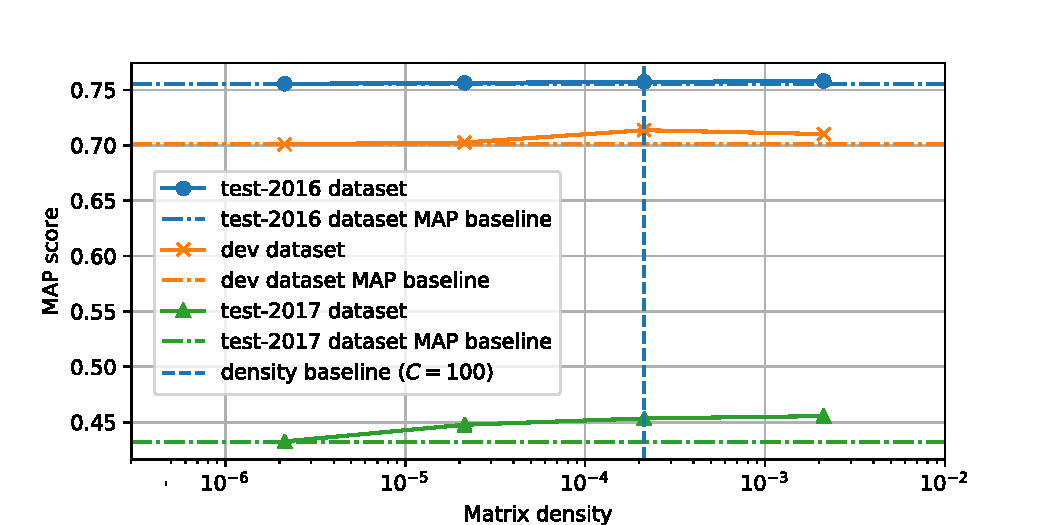
\includegraphics[trim={0.6cm 0.1cm 1.5cm 1.0cm}, scale=0.75]{figs/fig4}
\caption[A \abbr{MAP}-density plot for matrix $\mathbf S_{\textrm{lev}}$
and parameter $C$]{The \abbr{MAP}\index{map@\protect\abbr{MAP}}
  score plotted against the density of the matrix $\mathbf S_{\textrm{lev}}$
  \index{.slev@$\mathbf S_{\textrm{lev}}$} as we increase the parameter $C$
  \index{.c@$C$} from the value of $1$ (leftmost) to the value of $1{,}000$
  (rightmost). For every dataset, the baseline \abbr{MAP} score
  corresponds to using the cosine as a measure of similarity between two
  documents. Baseline density corresponds to the default value of~$C$.}
  \label{fig:similarity-fig4}
\end{figure}

\begin{figure}[p]
\centering%
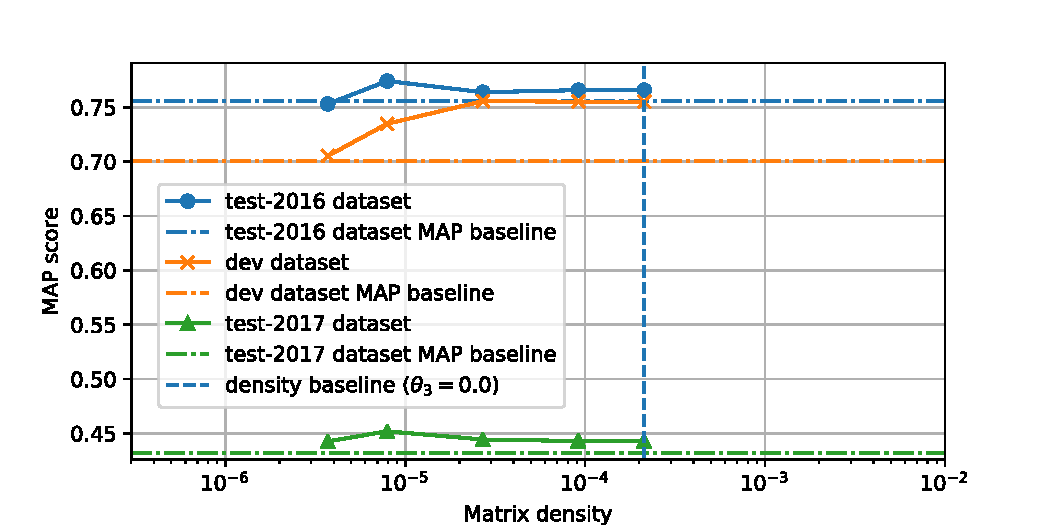
\includegraphics[trim={0.6cm 0.1cm 1.5cm 1.0cm}, scale=0.75]{figs/fig5}
\caption[A \abbr{MAP}-density plot for matrix $\mathbf S_{\textrm{lev}}$
and parameter $\theta_3$]{The
  \abbr{MAP}\index{map@\protect\abbr{MAP}} score plotted against the density of
  the matrix $\mathbf S_{\textrm{lev}}$ \index{.slev@$\mathbf S_{\textrm{lev}}$}
  as we increase the parameter $\theta_3$\index{.h3@$\theta_3$} from
  the value of $0.8$ (leftmost) to the value of $0$ (rightmost). For every
  dataset, the baseline \abbr{MAP} score corresponds to using the cosine as a measure
  of similarity between two documents. Baseline density corresponds to the
  default value~of~$\theta_3$.}
  \label{fig:similarity-fig5}
\end{figure}

\begin{figure}[p]
\centering%
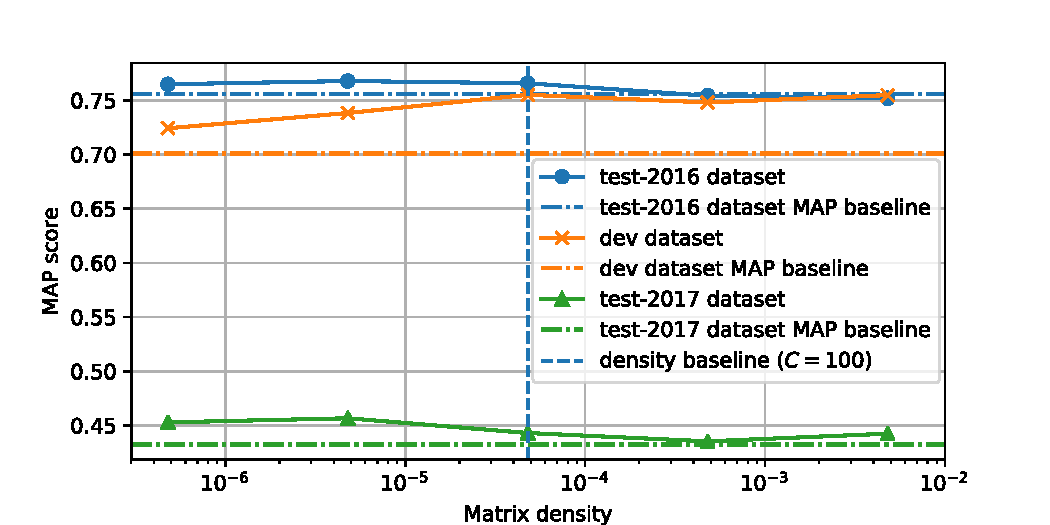
\includegraphics[trim={0.6cm 0.1cm 1.5cm 1.0cm}, scale=0.75]{figs/fig2}
\caption[A \abbr{MAP}-density plot for matrix $\mathbf S_{\textrm{rel}}$
and parameter $C$]{The \abbr{MAP}\index{map@\protect\abbr{MAP}}
  score plotted against the density of the matrix $\mathbf S_{\textrm{rel}}$
  \index{.srel@$\mathbf  S_{\textrm  {rel}}$} as we increase the parameter $C$
  \index{.c@$C$} from the value of $1$ (leftmost) to the value of $10{,}000$
  (rightmost). For every dataset, the baseline \abbr{MAP} score
  corresponds to using the cosine as a measure of similarity between two
  documents. Baseline density corresponds to the default value~of~$C$.}
  \label{fig:similarity-fig2}
\end{figure}

\begin{figure}[p]
\centering%
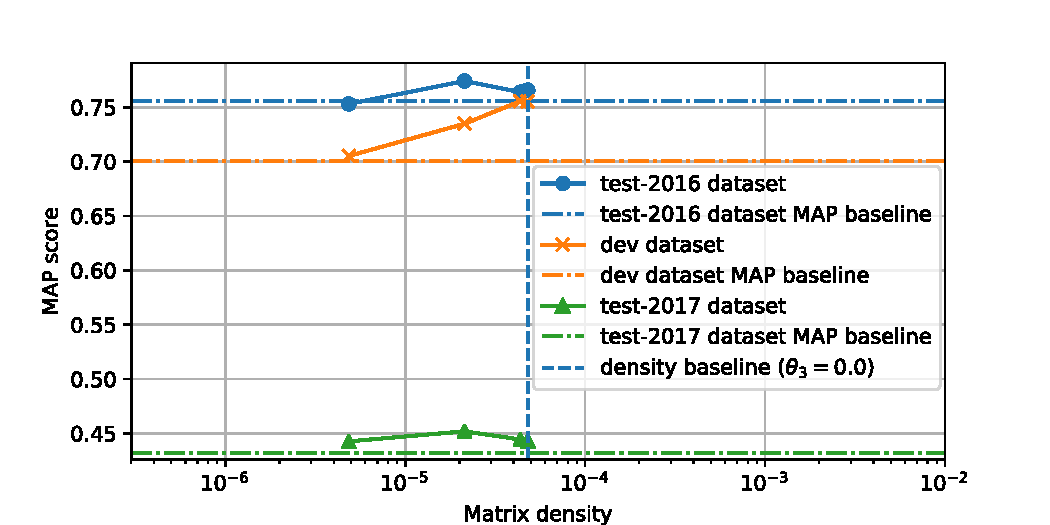
\includegraphics[trim={0.6cm 0.1cm 1.5cm 1.0cm}, scale=0.75]{figs/fig3}
\caption[A \abbr{MAP}-density plot for matrix $\mathbf S_{\textrm{rel}}$
and parameter $\theta_3$]{The
  \abbr{MAP}\index{map@\protect\abbr{MAP}} score plotted against the density of
  the matrix $\mathbf S_{\textrm{rel}}$ \index{.srel@$\mathbf S_{\textrm{rel}}$}
  as we increase the parameter $\theta_3$\index{.h3@$\theta_3$} from
  the value of $0.8$ (leftmost) to the value of $0.2$ (rightmost). For every
  dataset, the baseline \abbr{MAP} score corresponds to using the cosine as a measure
  of similarity between two documents. Baseline density corresponds to the
  default value~of~$\theta_3$.}
  \label{fig:similarity-fig3}
\end{figure}

\begin{figure}[tb]
\centering%
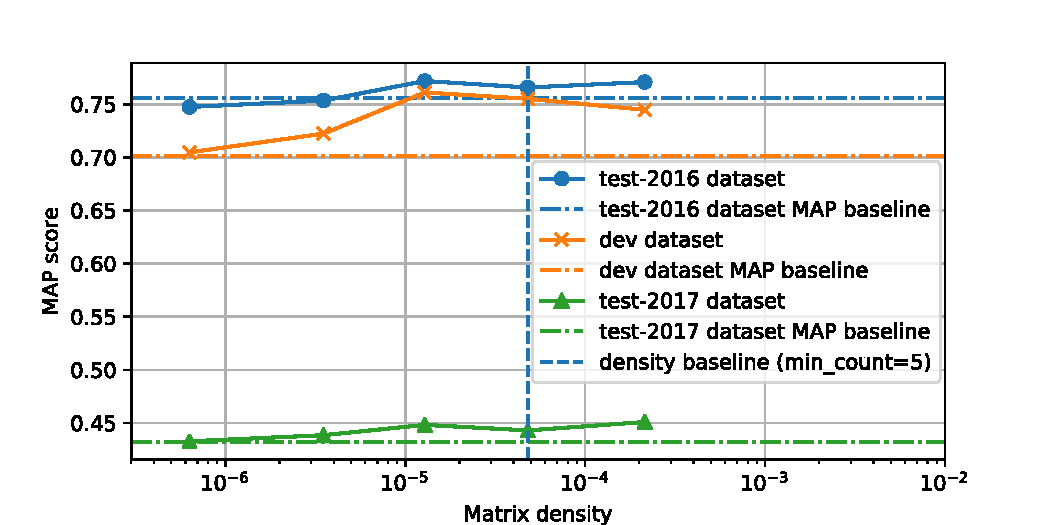
\includegraphics[trim={0.6cm 0.1cm 1.5cm 1.0cm}, scale=0.75]{figs/fig1}
\caption[A \abbr{MAP}-density plot for matrix $\mathbf S_{\textrm{rel}}$
and parameter \texttt{min\_count}]{The
  \abbr{MAP}\index{map@\protect\abbr{MAP}} score plotted against the density of
  the matrix $\mathbf S_{\textrm{rel}}$\index{.srel@$\mathbf S_{\textrm{rel}}$}
  as we increase the parameter
  \texttt{min\_count}\index{.mincount@\texttt{min\_count}} from the value of
  $5{,}000$ (leftmost) to the value of $0$ (rightmost). For every
  dataset, the baseline \abbr{MAP} score corresponds to using the cosine as a
  measure of similarity between two documents. Baseline density corresponds to
  the default value of \texttt{min\_count}.}
  \label{fig:similarity-fig1}
\end{figure}

\section{Results}
\label{sec:similarity-results}
By looking at \abbr{MAP}\index{map@\abbr {MAP}}-density plots of matrices
$\mathbf S_{\textrm{lev}}$ and $\mathbf S_{\textrm{rel}}$
\index{.slev@$\mathbf  S_{\textrm  {lev}}$}
\index{.srel@$\mathbf  S_{\textrm  {rel}}$}
in figures~\ref{fig:similarity-fig4}--\ref{fig:similarity-fig1},
several patterns emerge. Adjusting the parameter $C$\index{.c@$C$} leads to
higher \abbr{MAP} scores that adjusting the parameter
$\theta_3$\index{.h3@$\theta _3$} does. Increasing the density of $\mathbf
S$\index{.s@$\mathbf S$} leads to small or no increase in \abbr{MAP}, which
suggests that the extended model\index{standard model!extended} quickly reaches
a saturation point after which additional density of $\mathbf S$ does not lead
to an improvement in quality.

Looking at the individual figures, figure~\ref{fig:similarity-fig5} shows that
with the matrix $\mathbf S_{\textrm{lev}}$, the
elements with a value of $s_{ij}$ below $0.4$ are of limited usefulness to the model.
Reintroducing these elements increases the density, but leads to no improvement
in the \abbr{MAP} score as evidenced by the flat right tails of the plotted
line segments.
Figure~\ref{fig:similarity-fig2} shows that the subtask~B dev and test datasets behave
very differently with respect to the parameter $C$\index{.c@$C$} for the
matrix $\mathbf S_{\textrm{rel}}$. Whereas the test datasets seem to benefit
from the sparsification of $\mathbf S$, the dev dataset follows a reverse trend
and consistently benefits from the increased density of $\mathbf S$.
Figure~\ref{fig:similarity-fig3} shows that with the matrix
$\mathbf S_{\textrm{rel}}$, all $C=100$ nearest neighbors $j$ of each term $i$
receive a value of $s_{ij}$ above $0.2$ and lower values of the parameter $\theta_3$
are therefore ineffective in further increasing the density of $\mathbf
S$\index{.s@$\mathbf S$}.
\index{.slev@$\mathbf  S_{\textrm  {lev}}$}
\index{.srel@$\mathbf  S_{\textrm  {rel}}$}

Considering the results in tables~\ref{tab:similarity-results-2016} and
\ref{tab:similarity-results-2017}, the highest rank across both subtask~B test datasets
was achieved by the ensemble matrix $\mathbf S_{\avg}$\index{.savg@$\mathbf
S_{\avg}$}. The matrices $\mathbf S_{\textrm{lev}}$ and
$\mathbf S_{\textrm{rel}}$\index{.slev@$\mathbf  S_{\textrm  {lev}}$}
\index{.srel@$\mathbf  S_{\textrm  {rel}}$} using default parameters
steadily outperformed the standard model.

The results for the models using soft cosine\index{cosine
similarity!soft} with hard normalization\index{normalization!hard} vary
wildly between the datasets; the most stable results were achieved with the
Google News Word2vec\index{Word2vec} term embedding\index{term embedding}
model, which stays within a $1.2$ \abbr{MAP}\index{map@\abbr {MAP}} score radius
around the matrices $\mathbf S_{\textrm{lev}}$ and $\mathbf
S_{\textrm{rel}}$\index{.slev@$\mathbf  S_{\textrm  {lev}}$}
\index{.srel@$\mathbf  S_{\textrm  {rel}}$} using default parameters. This
shows that the query expansion approach described in
section~\ref{sec:similarity-inverted-index} is in general not inferior to
soft cosine similarity with soft normalization and can be used to implement
the extended model~\index{standard model!extended} in a way that allows us to
update $\mathbf S$\index{.s@$\mathbf S$} over time without reindexing the
document collection. Using just the inner product instead of soft cosine
similarity in the context of section~\ref{sec:similarity-vector-db} shows
promise on the 2016 test dataset, but performs poorly in the 2017 test dataset.

\section{Conclusion and future work}
\label{sec:similarity-conclusion}
In this chapter, I developed an extension to the standard model\index{standard
model} for modeling synonymy and I showed that is outperforms the standard
model on the text similarity task in the context of \abbr{QA}. Importantly, I
also showed that, unlike other models such as \index{LSA@\abbr{LSA}}\abbr{LSA}, a close
approximation of the described model can be implemented in a way that allows us
to update $\mathbf S$\index{.s@$\mathbf S$} over time without reindexing the
document collection. I also developed several matrices that model different
facets of term similarity; this is in contrast to models such as \abbr{LSA},
which are confined to a single measure of similarity such as term
co-occurences\index{term co-occurence}.

The discussion in section~\ref{sec:similarity-complexity} showed that little is
known about the density of the change-of-basis matrix \index{.e@$\mathbf E$}
and of the vectors that were cast to the orthonormal basis
$\bm\delta$\index{.d@$\bm\delta$}. In section~\ref{sec:similarity-measures}, I
introduced the notion of supervised ensemble term similarity matrices, but no
concrete implementation was described and evaluated. These are both fruitful
venues for future work.

\FloatBarrier

\begin{sidewaystable}[p]
\pagestyle{empty}
\index{.srel@$\mathbf  S_{\textrm  {rel}}$}
\index{.slev@$\mathbf  S_{\textrm  {lev}}$}
\index{.savg@$\mathbf S_{\avg}$}
\index{.h3@$\theta _3$}
\index{.c@$C$}
\index{normalization!hard}
\index{normalization!soft}
\index{cosine similarity!soft}
\index{cosine similarity}
\centering
\begin{liningfigs}
\footnotesize
\begin{tabular}{llllrlrl}
Matrix $\mathbf S$ &
  Term embedding model &
  Normalization &
  Measure &
  $C$ &
  $\theta_3$ &
  \texttt{min\_count} &
  \abbr{MAP}\index{map@\abbr {MAP}} \\ \toprule
$\mathbf S_{\textrm{rel}}$ & w2v.ql & soft & soft cosine & $100$ & $0.6$ & $5$ & $77.41$ \\
$\mathbf S_{\textrm{rel}}$ & w2v.ql & soft & soft cosine & $100$ & $0$ & $50$ & $77.18$ \\
$\mathbf S_{\textrm{rel}}$ & w2v.ql & hard & soft cosine & $100$ & $0$ & $5$ & $77.10$ \\
$\mathbf S_{\textrm{rel}}$ & w2v.ql & soft & soft cosine & $100$ & $0$ & $0$ & $77.08$ \\
$\mathbf S_{\textrm{rel}}$ & w2v.ql & soft & soft cosine & $10$ & $0$ & $5$ & $76.78$ \\
\multicolumn{4}{l}{\bfseries SemEval-2016 task~3 subtask~B winner (\abbr{UH-PRHLT}-primary)} &
  --- &
  --- &
  --- &
  \bfseries76.70 \\
$\mathbf S_{\textrm{avg}}$ & w2v.ql & soft & soft cosine & $100$ & $0$ & $5$ & $76.61$ \\
$\mathbf S_{\textrm{rel}}$ & w2v.ql & soft & soft cosine & $100$ & $0.2$ & $5$ & $76.57$ \\
$\mathbf S_{\textrm{rel}}$ & w2v.ql & soft & soft cosine & $100$ & $0$ & $5$ & $76.57$ \\ % charlet
$\mathbf S_{\textrm{rel}}$ & w2v.ql & soft & soft cosine & $1$ & $0$ & $5$ & $76.48$ \\
$\mathbf S_{\textrm{rel}}$ & w2v.ql & soft & soft cosine & $100$ & $0.4$ & $5$ & $76.38$ \\
$\mathbf S_{\textrm{lev}}$ & --- & soft & soft cosine & $100$ & $0.4$ & --- & $75.88$ \\
$\mathbf S_{\textrm{lev}}$ & --- & soft & soft cosine & $100$ & $0.6$ & --- & $75.81$ \\
$\mathbf S_{\textrm{lev}}$ & --- & soft & soft cosine & $1000$ & $0$ & --- & $75.80$ \\
$\mathbf S_{\textrm{rel}}$ & w2v.ql & --- & inner product & $100$ & $0$ & $5$ & $75.79$ \\
$\mathbf S_{\textrm{lev}}$ & --- & soft & soft cosine & $100$ & $0.2$ & --- & $75.72$ \\
$\mathbf S_{\textrm{lev}}$ & --- & soft & soft cosine & $100$ & $0$ & --- & $75.72$ \\
$\mathbf S_{\textrm{lev}}$ & --- & soft & soft cosine & $100$ & $0.8$ & --- & $75.67$ \\
$\mathbf S_{\textrm{rel}}$ & w2v.googlenews & hard & soft cosine & $100$ & $0$ & $5$ & $75.64$ \\
$\mathbf S_{\textrm{lev}}$ & --- & soft & soft cosine & $10$ & $0$ & --- & $75.63$ \\
$\mathbf S_{\textrm{lev}}$ & --- & soft & soft cosine & $1$ & $0$ & --- & $75.55$ \\
--- & --- & --- & \bfseries cosine & --- & --- & --- & \bfseries 75.55 \\
$\mathbf S_{\textrm{rel}}$ & w2v.ql & soft & soft cosine & $1000$ & $0$ & $5$ & $75.42$ \\
$\mathbf S_{\textrm{rel}}$ & glove.common\_crawl & hard & soft cosine & $100$ & $0$ & $5$ & $75.42$ \\
$\mathbf S_{\textrm{rel}}$ & w2v.ql & soft & soft cosine & $100$ & $0$ & $500$ & $75.34$ \\
$\mathbf S_{\textrm{rel}}$ & w2v.ql & soft & soft cosine & $100$ & $0.8$ & $5$ & $75.30$ \\
$\mathbf S_{\textrm{rel}}$ & w2v.ql & soft & soft cosine & $10000$ & $0$ & $5$ & $75.19$ \\
\multicolumn{3}{l}{\bfseries SemEval-2016 task~3 subtask~B \abbr{IR}\index{ir@\protect\abbr{IR}} baseline} &
  --- &
  --- &
  --- &
  --- &
  \bfseries74.75 \\
$\mathbf S_{\textrm{rel}}$ & w2v.ql & soft & soft cosine & $100$ & $0$ & $5000$ & $74.74$ \\
$\mathbf S_{\textrm{rel}}$ & fasttext.enwiki & hard & soft cosine & $100$ & $0$ & $5$ & $74.73$ \\
$\mathbf S_{\textrm{rel}}$ & glove.enwiki\_gigaword5 & hard & soft cosine & $100$ & $0$ & $5$ & $72.78$ \\
\end{tabular}
\end{liningfigs}
\caption[Results for all configurations on the SemEval-2016 task~3
subtask~B test dataset]{%
  Results for all configurations on the 2016 subtask~B test dataset.
  Baselines are highlighted~in~bold.}
\label{tab:similarity-results-2016}
\end{sidewaystable}

\begin{sidewaystable}[p]
\pagestyle{empty}
\index{.srel@$\mathbf  S_{\textrm  {rel}}$}
\index{.slev@$\mathbf  S_{\textrm  {lev}}$}
\index{.savg@$\mathbf S_{\avg}$}
\index{normalization!hard}
\index{normalization!soft}
\index{cosine similarity!soft}
\index{cosine similarity}
\index{.h3@$\theta _3$}
\index{.c@$C$}
\centering
\begin{liningfigs}
\footnotesize
\begin{tabular}{llllrlrl}
Matrix $\mathbf S$ &
  Term embedding model &
  Normalization &
  Measure &
  $C$ &
  $\theta_3$ &
  \texttt{min\_count} &
  \abbr{MAP}\index{map@\abbr {MAP}} \\ \toprule
\multicolumn{4}{l}{\bfseries SemEval-2017 task~3 subtask~B winner (SimBow-primary)} &
  --- &
  --- &
  --- &
  \bfseries47.22 \\
$\mathbf S_{\textrm{avg}}$ & w2v.ql & soft & soft cosine & $100$ & $0$ & $5$ & $46.04$ \\
$\mathbf S_{\textrm{rel}}$ & w2v.ql & soft & soft cosine & $10$ & $0$ & $5$ & $45.67$ \\
$\mathbf S_{\textrm{lev}}$ & --- & soft & soft cosine & $1000$ & $0$ & --- & $45.55$ \\
$\mathbf S_{\textrm{rel}}$ & glove.common\_crawl & hard & soft cosine & $100$ & $0$ & $5$ & $45.49$ \\
$\mathbf S_{\textrm{lev}}$ & --- & soft & soft cosine & $100$ & $0.6$ & --- & $45.35$ \\
$\mathbf S_{\textrm{lev}}$ & --- & soft & soft cosine & $100$ & $0.0$ & --- & $45.34$ \\
$\mathbf S_{\textrm{lev}}$ & --- & soft & soft cosine & $100$ & $0.2$ & --- & $45.31$ \\
$\mathbf S_{\textrm{rel}}$ & w2v.ql & soft & soft cosine & $1$ & $0$ & $5$ & $45.29$ \\
$\mathbf S_{\textrm{lev}}$ & --- & soft & soft cosine & $100$ & $0.4$ & --- & $45.22$ \\
$\mathbf S_{\textrm{rel}}$ & w2v.ql & soft & soft cosine & $100$ & $0.6$ & $5$ & $45.20$ \\
$\mathbf S_{\textrm{rel}}$ & glove.enwiki\_gigaword5 & hard & soft cosine & $100$ & $0$ & $5$ & $45.13$ \\
$\mathbf S_{\textrm{rel}}$ & w2v.ql & soft & soft cosine & $100$ & $0$ & $0$ & $45.10$ \\
$\mathbf S_{\textrm{rel}}$ & fasttext.enwiki & hard & soft cosine & $100$ & $0$ & $5$ & $44.94$ \\
$\mathbf S_{\textrm{rel}}$ & w2v.ql & soft & soft cosine & $100$ & $0$ & $50$ & $44.83$ \\
$\mathbf S_{\textrm{lev}}$ & --- & soft & soft cosine & $10$ & $0$ & --- & $44.77$ \\
$\mathbf S_{\textrm{lev}}$ & --- & soft & soft cosine & $100$ & $0.8$ & --- & $44.65$ \\
$\mathbf S_{\textrm{rel}}$ & w2v.ql & soft & soft cosine & $100$ & $0.4$ & $5$ & $44.45$ \\
$\mathbf S_{\textrm{rel}}$ & w2v.ql & soft & soft cosine & $100$ & $0.2$ & $5$ & $44.31$ \\
$\mathbf S_{\textrm{rel}}$ & w2v.ql & soft & soft cosine & $100$ & $0$ & $5$ & $44.31$ \\
$\mathbf S_{\textrm{rel}}$ & w2v.ql & soft & soft cosine & $100$ & $0.8$ & $5$ & $44.28$ \\
$\mathbf S_{\textrm{rel}}$ & w2v.ql & soft & soft cosine & $10000$ & $0$ & $5$ & $44.25$ \\
$\mathbf S_{\textrm{rel}}$ & w2v.googlenews & hard & soft cosine & $100$ & $0$ & $5$ & $44.13$ \\
$\mathbf S_{\textrm{rel}}$ & w2v.ql & soft & soft cosine & $100$ & $0$ & $500$ & $43.86$ \\
$\mathbf S_{\textrm{rel}}$ & w2v.ql & hard & soft cosine & $100$ & $0$ & $5$ & $43.76$ \\
$\mathbf S_{\textrm{rel}}$ & w2v.ql & soft & soft cosine & $1000$ & $0$ & $5$ & $43.54$ \\
$\mathbf S_{\textrm{rel}}$ & w2v.ql & soft & soft cosine & $100$ & $0$ & $5000$ & $43.28$ \\
$\mathbf S_{\textrm{lev}}$ & --- & soft & soft cosine & $1$ & $0$ & --- & $43.27$ \\
--- & --- & --- & \bfseries cosine & --- & --- & --- & \bfseries 43.25 \\
$\mathbf S_{\textrm{rel}}$ & w2v.ql & --- & inner product & $100$ & $0$ & $5$ & $42.17$ \\
\multicolumn{3}{l}{\bfseries SemEval-2017 task~3 subtask~B \abbr{IR}\index{ir@\protect\abbr{IR}} baseline} &
  --- &
  --- &
  --- &
  --- &
  \bfseries41.85 \\
\end{tabular}
\end{liningfigs}
\caption[Results for all configurations on the SemEval-2017 task~3
subtask~B test dataset]{%
  Results for all configurations on the 2017 subtask~B test dataset.
  Baselines are highlighted~in~bold.}
\label{tab:similarity-results-2017}
\end{sidewaystable}

\chapter{Conclusion}
\label{chap:conclusion}
In this work, I developed two models based on the standard vector space
bag-of-words\index{bag-of-words} model\index{standard model}. Both models were
described in mathematical terms, reviewed from the implementation standpoint,
and evaluated on the SemEval-2016 and 2017 task~3 datasets.

The first model exploits the fact that modern text retrieval systems employ
text segmentation during the indexing of documents. Using this knowledge, the
model achieves state-of-the-art results on our datasets.

The second model captures the similarity between different terms. Different
facets of synonymy can be modeled and changes to the similarity relations do
not require the reindexing of a document collection. The model surpasses the
standard vector space bag-of-words\index{bag-of-words} model\index{standard
model} on our datasets.

Since both models are mutually independent and each exploits a distinct
concept, they can be both implemented in a single \abbr{IR}\index{ir@\abbr {IR}} system.

\ifreview\else
\subsection*{Acknowledgments}
\abbr{\noexpand\MakeUppercase TAČR} Omega grant \abbr{TD03000295} is gratefully acknowledged.
\fi

%% The following section corresponds to the bibliography:
\nocite{ir:Zezula2006} %% The recommended literature.
\nocite{ml:IntroIR2008}
\nocite{mikolov2013efficient}
\begingroup\sloppy
\printbibliography[heading=bibintoc]
\endgroup

%% The following section corresponds to the index:
\makeatletter\thesis@blocks@clear\makeatother
\phantomsection %% Print the index and insert it into the
\addcontentsline{toc}{chapter}{\indexname} %% table of contents.
\printindex

\iffalse
\appendix %% Start the appendices.
\chapter{An appendix}
Here you can insert the appendices of your thesis.
\fi
\end{document}
